\documentclass[11pt]{article}
    \usepackage{ctex}
    \usepackage[breakable]{tcolorbox}
    \usepackage{parskip} % Stop auto-indenting (to mimic markdown behaviour)
    \usepackage{tabularx}
    \usepackage{multirow}
    \usepackage{makecell}
    \usepackage{subfigure}
    % Basic figure setup, for now with no caption control since it's done
    % automatically by Pandoc (which extracts ![](path) syntax from Markdown).
    \usepackage{graphicx}
    % Maintain compatibility with old templates. Remove in nbconvert 6.0
    \let\Oldincludegraphics\includegraphics
    % Ensure that by default, figures have no caption (until we provide a
    % proper Figure object with a Caption API and a way to capture that
    % in the conversion process - todo).


    \usepackage{float}
    \floatplacement{figure}{H} % forces figures to be placed at the correct location
    \usepackage{xcolor} % Allow colors to be defined
    \usepackage{enumerate} % Needed for markdown enumerations to work
    \usepackage{geometry} % Used to adjust the document margins
    \usepackage{amsmath} % Equations
    \usepackage{amssymb} % Equations
    \usepackage{textcomp} % defines textquotesingle
    % Hack from http://tex.stackexchange.com/a/47451/13684:
    \AtBeginDocument{%
        \def\PYZsq{\textquotesingle}% Upright quotes in Pygmentized code
    }
    \usepackage{upquote} % Upright quotes for verbatim code
    \usepackage{eurosym} % defines \euro

    \usepackage{iftex}
    \ifPDFTeX
        \usepackage[T1]{fontenc}
        \IfFileExists{alphabeta.sty}{
              \usepackage{alphabeta}
          }{
              \usepackage[mathletters]{ucs}
              \usepackage[utf8x]{inputenc}
          }
    \else
        \usepackage{fontspec}
        \usepackage{unicode-math}
    \fi

    \usepackage{fancyvrb} % verbatim replacement that allows latex
    \usepackage{grffile} % extends the file name processing of package graphics
                         % to support a larger range
    \makeatletter % fix for old versions of grffile with XeLaTeX
    \@ifpackagelater{grffile}{2019/11/01}
    {
      % Do nothing on new versions
    }
    {
      \def\Gread@@xetex#1{%
        \IfFileExists{"\Gin@base".bb}%
        {\Gread@eps{\Gin@base.bb}}%
        {\Gread@@xetex@aux#1}%
      }
    }
    \makeatother
    \usepackage[Export]{adjustbox} % Used to constrain images to a maximum size
    \adjustboxset{max size={0.9\linewidth}{0.9\paperheight}}

    % The hyperref package gives us a pdf with properly built
    % internal navigation ('pdf bookmarks' for the table of contents,
    % internal cross-reference links, web links for URLs, etc.)
    \usepackage{hyperref}
    % The default LaTeX title has an obnoxious amount of whitespace. By default,
    % titling removes some of it. It also provides customization options.
    \usepackage{titling}
    \usepackage{longtable} % longtable support required by pandoc >1.10
    \usepackage{booktabs}  % table support for pandoc > 1.12.2
    \usepackage{array}     % table support for pandoc >= 2.11.3
    \usepackage{calc}      % table minipage width calculation for pandoc >= 2.11.1
    \usepackage[inline]{enumitem} % IRkernel/repr support (it uses the enumerate* environment)
    \usepackage[normalem]{ulem} % ulem is needed to support strikethroughs (\sout)
                                % normalem makes italics be italics, not underlines
    \usepackage{mathrsfs}
    

    
    % Colors for the hyperref package
    \definecolor{urlcolor}{rgb}{0,.145,.698}
    \definecolor{linkcolor}{rgb}{.71,0.21,0.01}
    \definecolor{citecolor}{rgb}{.12,.54,.11}

    % ANSI colors
    \definecolor{ansi-black}{HTML}{3E424D}
    \definecolor{ansi-black-intense}{HTML}{282C36}
    \definecolor{ansi-red}{HTML}{E75C58}
    \definecolor{ansi-red-intense}{HTML}{B22B31}
    \definecolor{ansi-green}{HTML}{00A250}
    \definecolor{ansi-green-intense}{HTML}{007427}
    \definecolor{ansi-yellow}{HTML}{DDB62B}
    \definecolor{ansi-yellow-intense}{HTML}{B27D12}
    \definecolor{ansi-blue}{HTML}{208FFB}
    \definecolor{ansi-blue-intense}{HTML}{0065CA}
    \definecolor{ansi-magenta}{HTML}{D160C4}
    \definecolor{ansi-magenta-intense}{HTML}{A03196}
    \definecolor{ansi-cyan}{HTML}{60C6C8}
    \definecolor{ansi-cyan-intense}{HTML}{258F8F}
    \definecolor{ansi-white}{HTML}{C5C1B4}
    \definecolor{ansi-white-intense}{HTML}{A1A6B2}
    \definecolor{ansi-default-inverse-fg}{HTML}{FFFFFF}
    \definecolor{ansi-default-inverse-bg}{HTML}{000000}

    % common color for the border for error outputs.
    \definecolor{outerrorbackground}{HTML}{FFDFDF}

    % commands and environments needed by pandoc snippets
    % extracted from the output of `pandoc -s`
    \providecommand{\tightlist}{%
      \setlength{\itemsep}{0pt}\setlength{\parskip}{0pt}}
    \DefineVerbatimEnvironment{Highlighting}{Verbatim}{commandchars=\\\{\}}
    % Add ',fontsize=\small' for more characters per line
    \newenvironment{Shaded}{}{}
    \newcommand{\KeywordTok}[1]{\textcolor[rgb]{0.00,0.44,0.13}{\textbf{{#1}}}}
    \newcommand{\DataTypeTok}[1]{\textcolor[rgb]{0.56,0.13,0.00}{{#1}}}
    \newcommand{\DecValTok}[1]{\textcolor[rgb]{0.25,0.63,0.44}{{#1}}}
    \newcommand{\BaseNTok}[1]{\textcolor[rgb]{0.25,0.63,0.44}{{#1}}}
    \newcommand{\FloatTok}[1]{\textcolor[rgb]{0.25,0.63,0.44}{{#1}}}
    \newcommand{\CharTok}[1]{\textcolor[rgb]{0.25,0.44,0.63}{{#1}}}
    \newcommand{\StringTok}[1]{\textcolor[rgb]{0.25,0.44,0.63}{{#1}}}
    \newcommand{\CommentTok}[1]{\textcolor[rgb]{0.38,0.63,0.69}{\textit{{#1}}}}
    \newcommand{\OtherTok}[1]{\textcolor[rgb]{0.00,0.44,0.13}{{#1}}}
    \newcommand{\AlertTok}[1]{\textcolor[rgb]{1.00,0.00,0.00}{\textbf{{#1}}}}
    \newcommand{\FunctionTok}[1]{\textcolor[rgb]{0.02,0.16,0.49}{{#1}}}
    \newcommand{\RegionMarkerTok}[1]{{#1}}
    \newcommand{\ErrorTok}[1]{\textcolor[rgb]{1.00,0.00,0.00}{\textbf{{#1}}}}
    \newcommand{\NormalTok}[1]{{#1}}

    % Additional commands for more recent versions of Pandoc
    \newcommand{\ConstantTok}[1]{\textcolor[rgb]{0.53,0.00,0.00}{{#1}}}
    \newcommand{\SpecialCharTok}[1]{\textcolor[rgb]{0.25,0.44,0.63}{{#1}}}
    \newcommand{\VerbatimStringTok}[1]{\textcolor[rgb]{0.25,0.44,0.63}{{#1}}}
    \newcommand{\SpecialStringTok}[1]{\textcolor[rgb]{0.73,0.40,0.53}{{#1}}}
    \newcommand{\ImportTok}[1]{{#1}}
    \newcommand{\DocumentationTok}[1]{\textcolor[rgb]{0.73,0.13,0.13}{\textit{{#1}}}}
    \newcommand{\AnnotationTok}[1]{\textcolor[rgb]{0.38,0.63,0.69}{\textbf{\textit{{#1}}}}}
    \newcommand{\CommentVarTok}[1]{\textcolor[rgb]{0.38,0.63,0.69}{\textbf{\textit{{#1}}}}}
    \newcommand{\VariableTok}[1]{\textcolor[rgb]{0.10,0.09,0.49}{{#1}}}
    \newcommand{\ControlFlowTok}[1]{\textcolor[rgb]{0.00,0.44,0.13}{\textbf{{#1}}}}
    \newcommand{\OperatorTok}[1]{\textcolor[rgb]{0.40,0.40,0.40}{{#1}}}
    \newcommand{\BuiltInTok}[1]{{#1}}
    \newcommand{\ExtensionTok}[1]{{#1}}
    \newcommand{\PreprocessorTok}[1]{\textcolor[rgb]{0.74,0.48,0.00}{{#1}}}
    \newcommand{\AttributeTok}[1]{\textcolor[rgb]{0.49,0.56,0.16}{{#1}}}
    \newcommand{\InformationTok}[1]{\textcolor[rgb]{0.38,0.63,0.69}{\textbf{\textit{{#1}}}}}
    \newcommand{\WarningTok}[1]{\textcolor[rgb]{0.38,0.63,0.69}{\textbf{\textit{{#1}}}}}


    % Define a nice break command that doesn't care if a line doesn't already
    % exist.
    \def\br{\hspace*{\fill} \\* }
    % Math Jax compatibility definitions
    \def\gt{>}
    \def\lt{<}
    \let\Oldtex\TeX
    \let\Oldlatex\LaTeX
    \renewcommand{\TeX}{\textrm{\Oldtex}}
    \renewcommand{\LaTeX}{\textrm{\Oldlatex}}
    % Document parameters
    % Document title
    \title{\Huge\textbf{{Micro:bit 生命游戏进阶\\
            Game of Life PLUS}}}
    \author{\large{王子宸\quad 化学与分子工程学院} \\
            \large{石城玮\quad 生命科学学院}}
    
    
    
    
    
% Pygments definitions
\makeatletter
\def\PY@reset{\let\PY@it=\relax \let\PY@bf=\relax%
    \let\PY@ul=\relax \let\PY@tc=\relax%
    \let\PY@bc=\relax \let\PY@ff=\relax}
\def\PY@tok#1{\csname PY@tok@#1\endcsname}
\def\PY@toks#1+{\ifx\relax#1\empty\else%
    \PY@tok{#1}\expandafter\PY@toks\fi}
\def\PY@do#1{\PY@bc{\PY@tc{\PY@ul{%
    \PY@it{\PY@bf{\PY@ff{#1}}}}}}}
\def\PY#1#2{\PY@reset\PY@toks#1+\relax+\PY@do{#2}}

\@namedef{PY@tok@w}{\def\PY@tc##1{\textcolor[rgb]{0.73,0.73,0.73}{##1}}}
\@namedef{PY@tok@c}{\let\PY@it=\textit\def\PY@tc##1{\textcolor[rgb]{0.24,0.48,0.48}{##1}}}
\@namedef{PY@tok@cp}{\def\PY@tc##1{\textcolor[rgb]{0.61,0.40,0.00}{##1}}}
\@namedef{PY@tok@k}{\let\PY@bf=\textbf\def\PY@tc##1{\textcolor[rgb]{0.00,0.50,0.00}{##1}}}
\@namedef{PY@tok@kp}{\def\PY@tc##1{\textcolor[rgb]{0.00,0.50,0.00}{##1}}}
\@namedef{PY@tok@kt}{\def\PY@tc##1{\textcolor[rgb]{0.69,0.00,0.25}{##1}}}
\@namedef{PY@tok@o}{\def\PY@tc##1{\textcolor[rgb]{0.40,0.40,0.40}{##1}}}
\@namedef{PY@tok@ow}{\let\PY@bf=\textbf\def\PY@tc##1{\textcolor[rgb]{0.67,0.13,1.00}{##1}}}
\@namedef{PY@tok@nb}{\def\PY@tc##1{\textcolor[rgb]{0.00,0.50,0.00}{##1}}}
\@namedef{PY@tok@nf}{\def\PY@tc##1{\textcolor[rgb]{0.00,0.00,1.00}{##1}}}
\@namedef{PY@tok@nc}{\let\PY@bf=\textbf\def\PY@tc##1{\textcolor[rgb]{0.00,0.00,1.00}{##1}}}
\@namedef{PY@tok@nn}{\let\PY@bf=\textbf\def\PY@tc##1{\textcolor[rgb]{0.00,0.00,1.00}{##1}}}
\@namedef{PY@tok@ne}{\let\PY@bf=\textbf\def\PY@tc##1{\textcolor[rgb]{0.80,0.25,0.22}{##1}}}
\@namedef{PY@tok@nv}{\def\PY@tc##1{\textcolor[rgb]{0.10,0.09,0.49}{##1}}}
\@namedef{PY@tok@no}{\def\PY@tc##1{\textcolor[rgb]{0.53,0.00,0.00}{##1}}}
\@namedef{PY@tok@nl}{\def\PY@tc##1{\textcolor[rgb]{0.46,0.46,0.00}{##1}}}
\@namedef{PY@tok@ni}{\let\PY@bf=\textbf\def\PY@tc##1{\textcolor[rgb]{0.44,0.44,0.44}{##1}}}
\@namedef{PY@tok@na}{\def\PY@tc##1{\textcolor[rgb]{0.41,0.47,0.13}{##1}}}
\@namedef{PY@tok@nt}{\let\PY@bf=\textbf\def\PY@tc##1{\textcolor[rgb]{0.00,0.50,0.00}{##1}}}
\@namedef{PY@tok@nd}{\def\PY@tc##1{\textcolor[rgb]{0.67,0.13,1.00}{##1}}}
\@namedef{PY@tok@s}{\def\PY@tc##1{\textcolor[rgb]{0.73,0.13,0.13}{##1}}}
\@namedef{PY@tok@sd}{\let\PY@it=\textit\def\PY@tc##1{\textcolor[rgb]{0.73,0.13,0.13}{##1}}}
\@namedef{PY@tok@si}{\let\PY@bf=\textbf\def\PY@tc##1{\textcolor[rgb]{0.64,0.35,0.47}{##1}}}
\@namedef{PY@tok@se}{\let\PY@bf=\textbf\def\PY@tc##1{\textcolor[rgb]{0.67,0.36,0.12}{##1}}}
\@namedef{PY@tok@sr}{\def\PY@tc##1{\textcolor[rgb]{0.64,0.35,0.47}{##1}}}
\@namedef{PY@tok@ss}{\def\PY@tc##1{\textcolor[rgb]{0.10,0.09,0.49}{##1}}}
\@namedef{PY@tok@sx}{\def\PY@tc##1{\textcolor[rgb]{0.00,0.50,0.00}{##1}}}
\@namedef{PY@tok@m}{\def\PY@tc##1{\textcolor[rgb]{0.40,0.40,0.40}{##1}}}
\@namedef{PY@tok@gh}{\let\PY@bf=\textbf\def\PY@tc##1{\textcolor[rgb]{0.00,0.00,0.50}{##1}}}
\@namedef{PY@tok@gu}{\let\PY@bf=\textbf\def\PY@tc##1{\textcolor[rgb]{0.50,0.00,0.50}{##1}}}
\@namedef{PY@tok@gd}{\def\PY@tc##1{\textcolor[rgb]{0.63,0.00,0.00}{##1}}}
\@namedef{PY@tok@gi}{\def\PY@tc##1{\textcolor[rgb]{0.00,0.52,0.00}{##1}}}
\@namedef{PY@tok@gr}{\def\PY@tc##1{\textcolor[rgb]{0.89,0.00,0.00}{##1}}}
\@namedef{PY@tok@ge}{\let\PY@it=\textit}
\@namedef{PY@tok@gs}{\let\PY@bf=\textbf}
\@namedef{PY@tok@gp}{\let\PY@bf=\textbf\def\PY@tc##1{\textcolor[rgb]{0.00,0.00,0.50}{##1}}}
\@namedef{PY@tok@go}{\def\PY@tc##1{\textcolor[rgb]{0.44,0.44,0.44}{##1}}}
\@namedef{PY@tok@gt}{\def\PY@tc##1{\textcolor[rgb]{0.00,0.27,0.87}{##1}}}
\@namedef{PY@tok@err}{\def\PY@bc##1{{\setlength{\fboxsep}{\string -\fboxrule}\fcolorbox[rgb]{1.00,0.00,0.00}{1,1,1}{\strut ##1}}}}
\@namedef{PY@tok@kc}{\let\PY@bf=\textbf\def\PY@tc##1{\textcolor[rgb]{0.00,0.50,0.00}{##1}}}
\@namedef{PY@tok@kd}{\let\PY@bf=\textbf\def\PY@tc##1{\textcolor[rgb]{0.00,0.50,0.00}{##1}}}
\@namedef{PY@tok@kn}{\let\PY@bf=\textbf\def\PY@tc##1{\textcolor[rgb]{0.00,0.50,0.00}{##1}}}
\@namedef{PY@tok@kr}{\let\PY@bf=\textbf\def\PY@tc##1{\textcolor[rgb]{0.00,0.50,0.00}{##1}}}
\@namedef{PY@tok@bp}{\def\PY@tc##1{\textcolor[rgb]{0.00,0.50,0.00}{##1}}}
\@namedef{PY@tok@fm}{\def\PY@tc##1{\textcolor[rgb]{0.00,0.00,1.00}{##1}}}
\@namedef{PY@tok@vc}{\def\PY@tc##1{\textcolor[rgb]{0.10,0.09,0.49}{##1}}}
\@namedef{PY@tok@vg}{\def\PY@tc##1{\textcolor[rgb]{0.10,0.09,0.49}{##1}}}
\@namedef{PY@tok@vi}{\def\PY@tc##1{\textcolor[rgb]{0.10,0.09,0.49}{##1}}}
\@namedef{PY@tok@vm}{\def\PY@tc##1{\textcolor[rgb]{0.10,0.09,0.49}{##1}}}
\@namedef{PY@tok@sa}{\def\PY@tc##1{\textcolor[rgb]{0.73,0.13,0.13}{##1}}}
\@namedef{PY@tok@sb}{\def\PY@tc##1{\textcolor[rgb]{0.73,0.13,0.13}{##1}}}
\@namedef{PY@tok@sc}{\def\PY@tc##1{\textcolor[rgb]{0.73,0.13,0.13}{##1}}}
\@namedef{PY@tok@dl}{\def\PY@tc##1{\textcolor[rgb]{0.73,0.13,0.13}{##1}}}
\@namedef{PY@tok@s2}{\def\PY@tc##1{\textcolor[rgb]{0.73,0.13,0.13}{##1}}}
\@namedef{PY@tok@sh}{\def\PY@tc##1{\textcolor[rgb]{0.73,0.13,0.13}{##1}}}
\@namedef{PY@tok@s1}{\def\PY@tc##1{\textcolor[rgb]{0.73,0.13,0.13}{##1}}}
\@namedef{PY@tok@mb}{\def\PY@tc##1{\textcolor[rgb]{0.40,0.40,0.40}{##1}}}
\@namedef{PY@tok@mf}{\def\PY@tc##1{\textcolor[rgb]{0.40,0.40,0.40}{##1}}}
\@namedef{PY@tok@mh}{\def\PY@tc##1{\textcolor[rgb]{0.40,0.40,0.40}{##1}}}
\@namedef{PY@tok@mi}{\def\PY@tc##1{\textcolor[rgb]{0.40,0.40,0.40}{##1}}}
\@namedef{PY@tok@il}{\def\PY@tc##1{\textcolor[rgb]{0.40,0.40,0.40}{##1}}}
\@namedef{PY@tok@mo}{\def\PY@tc##1{\textcolor[rgb]{0.40,0.40,0.40}{##1}}}
\@namedef{PY@tok@ch}{\let\PY@it=\textit\def\PY@tc##1{\textcolor[rgb]{0.24,0.48,0.48}{##1}}}
\@namedef{PY@tok@cm}{\let\PY@it=\textit\def\PY@tc##1{\textcolor[rgb]{0.24,0.48,0.48}{##1}}}
\@namedef{PY@tok@cpf}{\let\PY@it=\textit\def\PY@tc##1{\textcolor[rgb]{0.24,0.48,0.48}{##1}}}
\@namedef{PY@tok@c1}{\let\PY@it=\textit\def\PY@tc##1{\textcolor[rgb]{0.24,0.48,0.48}{##1}}}
\@namedef{PY@tok@cs}{\let\PY@it=\textit\def\PY@tc##1{\textcolor[rgb]{0.24,0.48,0.48}{##1}}}

\def\PYZbs{\char`\\}
\def\PYZus{\char`\_}
\def\PYZob{\char`\{}
\def\PYZcb{\char`\}}
\def\PYZca{\char`\^}
\def\PYZam{\char`\&}
\def\PYZlt{\char`\<}
\def\PYZgt{\char`\>}
\def\PYZsh{\char`\#}
\def\PYZpc{\char`\%}
\def\PYZdl{\char`\$}
\def\PYZhy{\char`\-}
\def\PYZsq{\char`\'}
\def\PYZdq{\char`\"}
\def\PYZti{\char`\~}
% for compatibility with earlier versions
\def\PYZat{@}
\def\PYZlb{[}
\def\PYZrb{]}
\makeatother


    % For linebreaks inside Verbatim environment from package fancyvrb.
    \makeatletter
        \newbox\Wrappedcontinuationbox
        \newbox\Wrappedvisiblespacebox
        \newcommand*\Wrappedvisiblespace {\textcolor{red}{\textvisiblespace}}
        \newcommand*\Wrappedcontinuationsymbol {\textcolor{red}{\llap{\tiny$\m@th\hookrightarrow$}}}
        \newcommand*\Wrappedcontinuationindent {3ex }
        \newcommand*\Wrappedafterbreak {\kern\Wrappedcontinuationindent\copy\Wrappedcontinuationbox}
        % Take advantage of the already applied Pygments mark-up to insert
        % potential linebreaks for TeX processing.
        %        {, <, #, %, $, ' and ": go to next line.
        %        _, }, ^, &, >, - and ~: stay at end of broken line.
        % Use of \textquotesingle for straight quote.
        \newcommand*\Wrappedbreaksatspecials {%
            \def\PYGZus{\discretionary{\char`\_}{\Wrappedafterbreak}{\char`\_}}%
            \def\PYGZob{\discretionary{}{\Wrappedafterbreak\char`\{}{\char`\{}}%
            \def\PYGZcb{\discretionary{\char`\}}{\Wrappedafterbreak}{\char`\}}}%
            \def\PYGZca{\discretionary{\char`\^}{\Wrappedafterbreak}{\char`\^}}%
            \def\PYGZam{\discretionary{\char`\&}{\Wrappedafterbreak}{\char`\&}}%
            \def\PYGZlt{\discretionary{}{\Wrappedafterbreak\char`\<}{\char`\<}}%
            \def\PYGZgt{\discretionary{\char`\>}{\Wrappedafterbreak}{\char`\>}}%
            \def\PYGZsh{\discretionary{}{\Wrappedafterbreak\char`\#}{\char`\#}}%
            \def\PYGZpc{\discretionary{}{\Wrappedafterbreak\char`\%}{\char`\%}}%
            \def\PYGZdl{\discretionary{}{\Wrappedafterbreak\char`\$}{\char`\$}}%
            \def\PYGZhy{\discretionary{\char`\-}{\Wrappedafterbreak}{\char`\-}}%
            \def\PYGZsq{\discretionary{}{\Wrappedafterbreak\textquotesingle}{\textquotesingle}}%
            \def\PYGZdq{\discretionary{}{\Wrappedafterbreak\char`\"}{\char`\"}}%
            \def\PYGZti{\discretionary{\char`\~}{\Wrappedafterbreak}{\char`\~}}%
        }
        % Some characters . , ; ? ! / are not pygmentized.
        % This macro makes them "active" and they will insert potential linebreaks
        \newcommand*\Wrappedbreaksatpunct {%
            \lccode`\~`\.\lowercase{\def~}{\discretionary{\hbox{\char`\.}}{\Wrappedafterbreak}{\hbox{\char`\.}}}%
            \lccode`\~`\,\lowercase{\def~}{\discretionary{\hbox{\char`\,}}{\Wrappedafterbreak}{\hbox{\char`\,}}}%
            \lccode`\~`\;\lowercase{\def~}{\discretionary{\hbox{\char`\;}}{\Wrappedafterbreak}{\hbox{\char`\;}}}%
            \lccode`\~`\:\lowercase{\def~}{\discretionary{\hbox{\char`\:}}{\Wrappedafterbreak}{\hbox{\char`\:}}}%
            \lccode`\~`\?\lowercase{\def~}{\discretionary{\hbox{\char`\?}}{\Wrappedafterbreak}{\hbox{\char`\?}}}%
            \lccode`\~`\!\lowercase{\def~}{\discretionary{\hbox{\char`\!}}{\Wrappedafterbreak}{\hbox{\char`\!}}}%
            \lccode`\~`\/\lowercase{\def~}{\discretionary{\hbox{\char`\/}}{\Wrappedafterbreak}{\hbox{\char`\/}}}%
            \catcode`\.\active
            \catcode`\,\active
            \catcode`\;\active
            \catcode`\:\active
            \catcode`\?\active
            \catcode`\!\active
            \catcode`\/\active
            \lccode`\~`\~
        }
    \makeatother

    \let\OriginalVerbatim=\Verbatim
    \makeatletter
    \renewcommand{\Verbatim}[1][1]{%
        %\parskip\z@skip
        \sbox\Wrappedcontinuationbox {\Wrappedcontinuationsymbol}%
        \sbox\Wrappedvisiblespacebox {\FV@SetupFont\Wrappedvisiblespace}%
        \def\FancyVerbFormatLine ##1{\hsize\linewidth
            \vtop{\raggedright\hyphenpenalty\z@\exhyphenpenalty\z@
                \doublehyphendemerits\z@\finalhyphendemerits\z@
                \strut ##1\strut}%
        }%
        % If the linebreak is at a space, the latter will be displayed as visible
        % space at end of first line, and a continuation symbol starts next line.
        % Stretch/shrink are however usually zero for typewriter font.
        \def\FV@Space {%
            \nobreak\hskip\z@ plus\fontdimen3\font minus\fontdimen4\font
            \discretionary{\copy\Wrappedvisiblespacebox}{\Wrappedafterbreak}
            {\kern\fontdimen2\font}%
        }%

        % Allow breaks at special characters using \PYG... macros.
        \Wrappedbreaksatspecials
        % Breaks at punctuation characters . , ; ? ! and / need catcode=\active
        \OriginalVerbatim[#1,codes*=\Wrappedbreaksatpunct]%
    }
    \makeatother

    % Exact colors from NB
    \definecolor{incolor}{HTML}{303F9F}
    \definecolor{outcolor}{HTML}{D84315}
    \definecolor{cellborder}{HTML}{CFCFCF}
    \definecolor{cellbackground}{HTML}{F7F7F7}

    % prompt
    \makeatletter
    \newcommand{\boxspacing}{\kern\kvtcb@left@rule\kern\kvtcb@boxsep}
    \makeatother
    \newcommand{\prompt}[4]{
        {\ttfamily\llap{{\color{#2}[#3]:\hspace{3pt}#4}}\vspace{-\baselineskip}}
    }
    

    
    % Prevent overflowing lines due to hard-to-break entities
    \sloppy
    % Setup hyperref package
    \hypersetup{
      breaklinks=true,  % so long urls are correctly broken across lines
      colorlinks=true,
      urlcolor=urlcolor,
      linkcolor=linkcolor,
      citecolor=citecolor,
      }
    % Slightly bigger margins than the latex defaults
    
    \geometry{verbose,tmargin=1in,bmargin=1in,lmargin=1in,rmargin=1in}
    
    

\begin{document}
    
    \maketitle
    
    \tableofcontents

    \setcounter{section}{-1}
    \hypertarget{ux6458ux8981}{%
\section{摘要}\label{ux6458ux8981}}

\hspace{2em}生命游戏是由英国数学家康威自主研发的一款开放世界冒险游戏。受到其启发,我们小组在原版生命游戏规则的基础上进行了一定的扩展,加入了更多的元素从而进一步模仿了生物的多样性,在此基础上,不同的元素遵循不同的基本变化原则,从而可以实现多种多样的变化,甚至在经过适当的组合以后,可以用于进行计算。我们采用了抽象,模拟,组合的方式,在\(5\times 5\)的Micro:bit上实现了这一系统。其结果深刻揭示了“涌现特征”的原理,系统的功能多于每一个组分的功能之和,在某种程度上复现了生命从简到繁的演化。

    \hypertarget{ux9009ux9898ux53caux521bux610fux4ecbux7ecd}{%
\section{选题及创意介绍}\label{ux9009ux9898ux53caux521bux610fux4ecbux7ecd}}

\hspace{2em} 生命游戏(Game of Life),是由英国数学家约翰霍顿康威于1970年设计的细胞自动机。这是一个零玩家游戏,这意味着它的进化是由它的初始状态决定的,不需要进一步的输入。人们通过创建初始配置并观察它如何演变来与生命游戏互动。它是图灵完备的,可以模拟通用构造函数或任何其他图灵机。

\hspace{2em} 生命游戏的宇宙是一个无限的二维正交网格,由方形细胞组成,每个细胞都处于两种可能的状态之一:生存或者死亡。每个像元都与其八个相邻的像元相互作用,这些像元是水平、垂直或对角线相邻的像元。在每个步骤中,每个细胞按照以下规则进行转换:
\begin{enumerate}
    \item 任何具有两个或三个活邻居的活细胞都能存活下来。
    \item 任何具有三个活邻居的死细胞都成为活细胞。
    \item 所有其他活细胞在下一代死亡。同样,所有其他死细胞都保持死亡状态。
\end{enumerate}

\hspace{2em} 初始模式构成了系统的种子。第一代是通过将上述规则同时应用于种子中的每个细胞来创建的,无论是活的还是死的。每一代都是前一代的纯函数。这些规则继续反复应用,以创造下一代。

\hspace{2em}考虑一种更为复杂的情形,将生命游戏的生存细胞种类由一种扩展为3种,且每种细胞分别具有一定的内禀属性:独立度、竞争力与扩散系数:
\begin{enumerate}
    \item \textbf{独立度}:用于衡量一种生存细胞对周围细胞的依赖度,若周围细胞总数小于依赖度,则细胞因孤独而死
    \item \textbf{竞争力}:用于衡量一种生存细胞,其周围的拥挤程度,如果周围细胞的总竞争力大于一常数,则细胞因拥挤而死
    \item \textbf{扩散系数}:用于衡量死亡细胞周围每种细胞的总扩散系数,按照竞争力由大到小的顺序,优先诞生竞争力大,且死亡细胞周围的该种竞争力的细胞的总扩散系数,大于该种竞争力细胞的独立度,则在死亡细胞的位置生成该种竞争力的细胞
\end{enumerate}

\hspace{2em}通过这样的方式将生命游戏的细胞演化跟更为复杂、生动而有趣。

\section{设计方案与硬件连接}

\subsection{设计方案}
\hspace{2em} 设计两种模式,分别对应简单生命游戏、复杂生命游戏:
\begin{itemize}
    \item \textbf{简单生命游戏}:按照康威生命游戏规则运行
    \item \textbf{复杂生命游戏}:含有三种生存细胞与一种死亡细胞,基于独立度、竞争力、扩散系数与扩散阈值演化的生命游戏
    \\
    \begin{table}[h] % 开始表格环境
      \centering % 居中
      \caption{\textbf{三种生存细胞的特性}} % 表格标题
      \begin{tabularx}{\linewidth}{X X m{6cm}} % 表格列宽自适应,并且有三列
            \hline \centering 细胞类型(对应显示亮度) & \centering 显示效果 & 细胞特性 \\
            \hline \centering \textbf{3} & \centering \begin{adjustbox}{valign=m}
                
\includegraphics[width=0.15\textwidth]{set3/3.png}
                \end{adjustbox} &  能够快速的繁殖, 对其他细胞抑制力弱, 但是只有周围有不少细胞才能存活\\
            \hline \centering \textbf{6} & \centering  \begin{adjustbox}{valign=m}
                
\includegraphics[width=0.15\textwidth]{set3/1.png}
                \end{adjustbox}  & 繁殖慢, 但是可以独立生存, 且会抑制周围细胞的生长 \\
            \hline \centering \textbf{9} & \centering \begin{adjustbox}{valign=m}
                
\includegraphics[width=0.15\textwidth]{set3/2.png}
                \end{adjustbox}  & 繁殖速度, 周围最适细胞数量, 对周围细胞的抑制力均中等  \\
            \hline
      \end{tabularx}
    \end{table}
\end{itemize}
\subsection{硬件连接}
\hspace{2em} 由于生命游戏并不需要除去Micro:bit之外的硬件,因此,使用\href{https://python.microbit.org/v/3}{Micro:bit官网}提供的在线Micro:bit进行模拟仿真实验。
    \hypertarget{ux5b9eux73b0ux65b9ux6848ux4e0eux4ee3ux7801ux5206ux6790}{%
\section{实现方案与代码分析}\label{ux5b9eux73b0ux65b9ux6848ux4e0eux4ee3ux7801ux5206ux6790}}

    \hypertarget{ux5b9eux73b0ux65b9ux6848}{%
\subsection{实现方案}\label{ux5b9eux73b0ux65b9ux6848}}

\hypertarget{ux6a21ux5f0fux9009ux62e9}{%
\subsubsection{模式选择}\label{ux6a21ux5f0fux9009ux62e9}}
\hspace{2em} 本程序分为两大模式,分别为:
\begin{enumerate}
    \item \textbf{简单模式 mod1}:实现康威生命游戏
    \item \textbf{复杂模式 mod2}:实现复杂生命游戏:
\end{enumerate}
\begin{figure}[h]
    \centering
    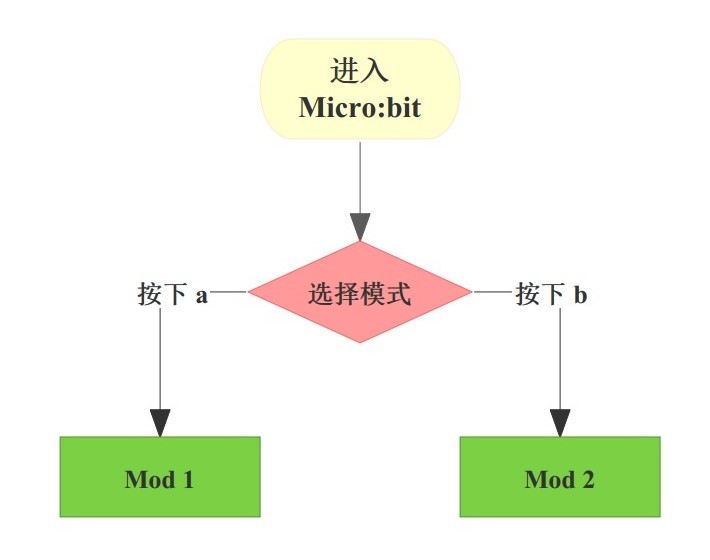
\includegraphics[width = .5\textwidth]{set1/1.jpg}
    \caption{\textbf{简单模式 mod1的实现流程}}
\end{figure}


\newpage
\subsubsection{\texorpdfstring{\texttt{mod1}与\texttt{mod2}的主流程实现}{mod1与mod2的主流程实现}}
\begin{figure}[H]
    \centering
    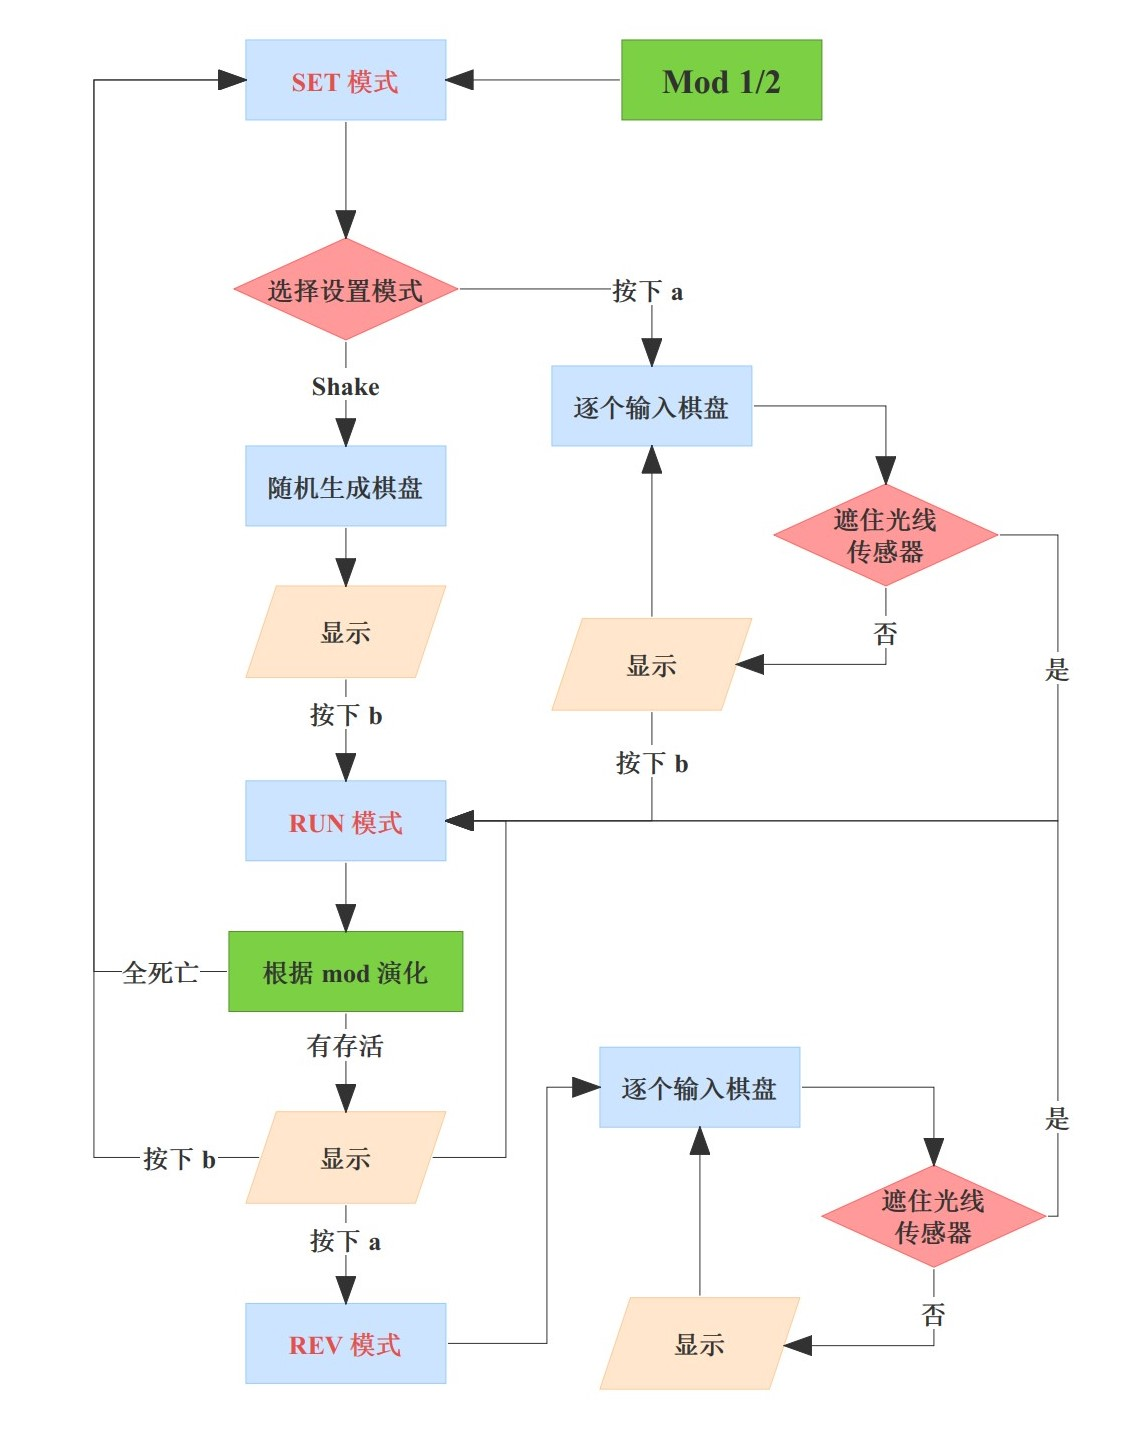
\includegraphics[width = \textwidth]{set1/2.jpg}
    \caption{\textbf{mod1与mod2主流程实现}}
\end{figure}


\hypertarget{mod1ux7b80ux5355ux6a21ux5f0f}{%
\subsubsection{\texorpdfstring{\texttt{mod1}:简单模式}{mod1:简单模式}}\label{mod1ux7b80ux5355ux6a21ux5f0f}}
\begin{itemize}

\item
  输入实现
\begin{figure}[H]
    \centering
    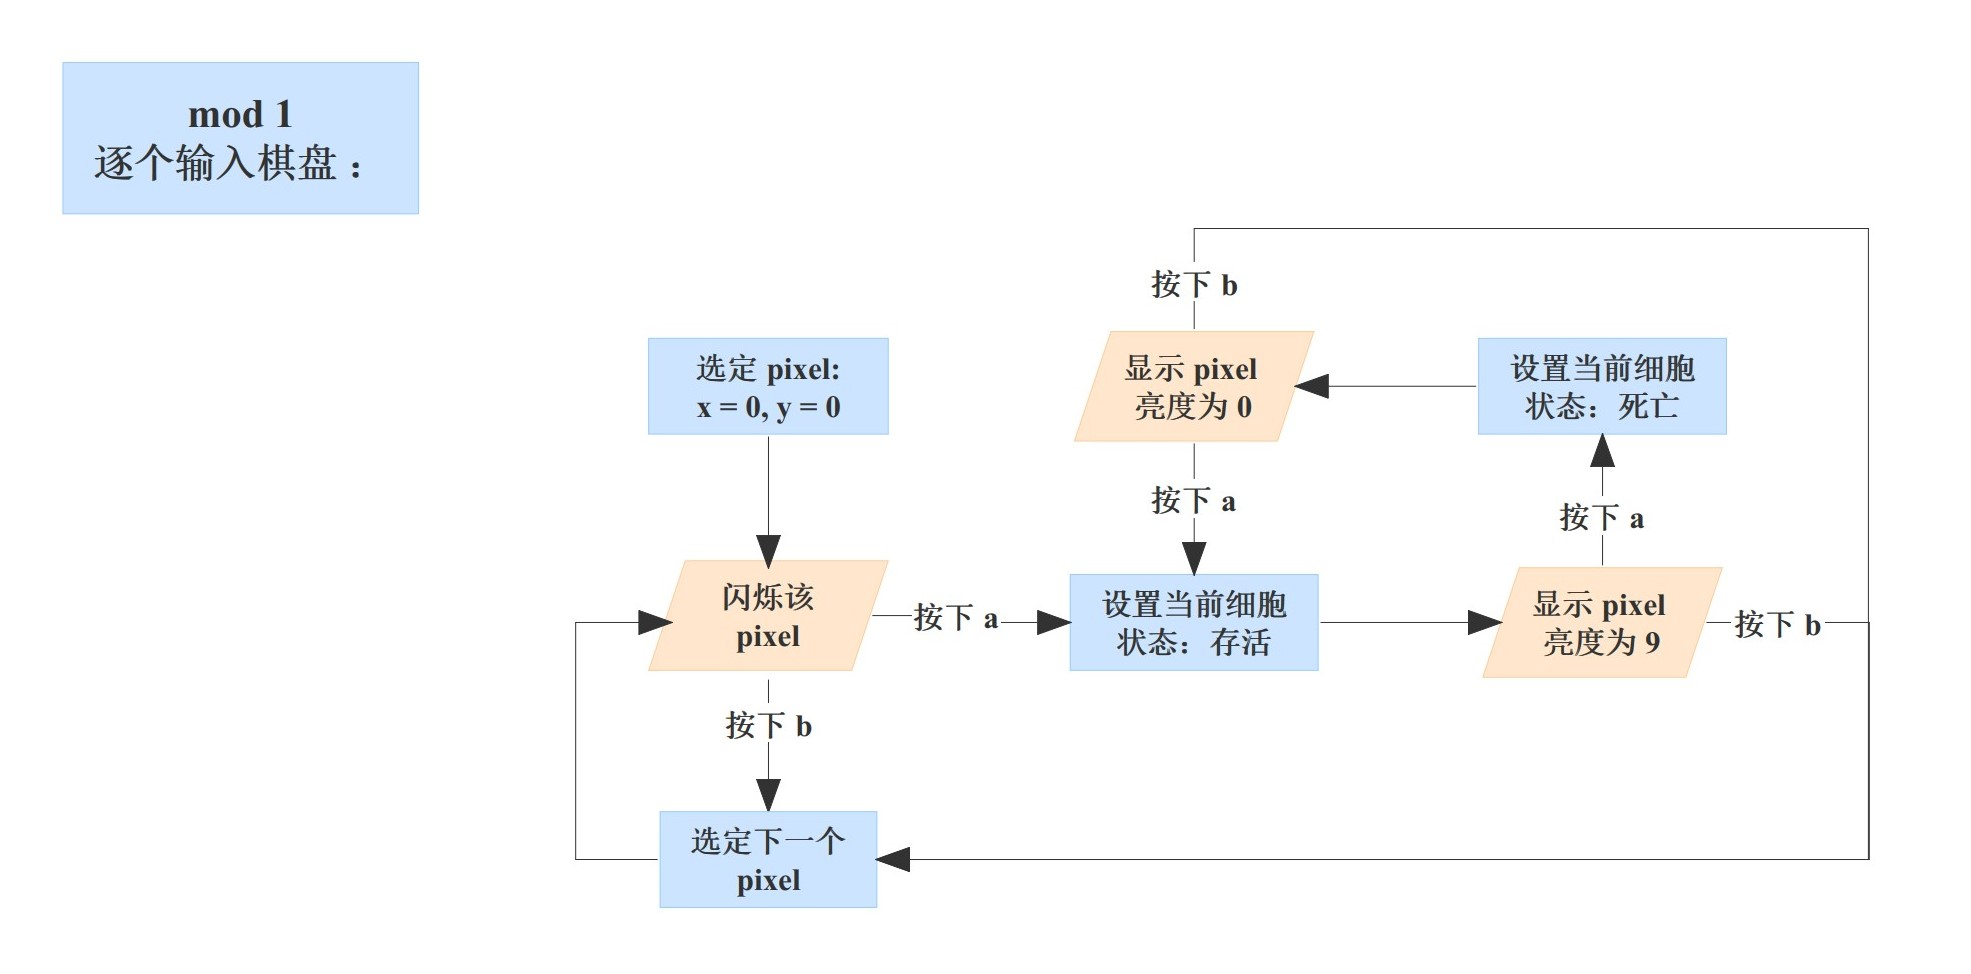
\includegraphics[width = 0.95\textwidth]{set1/5.jpg}
    \caption{\textbf{mod1 的输入实现}}
\end{figure}
\item 
  
\begin{figure}[H]
    \centering
    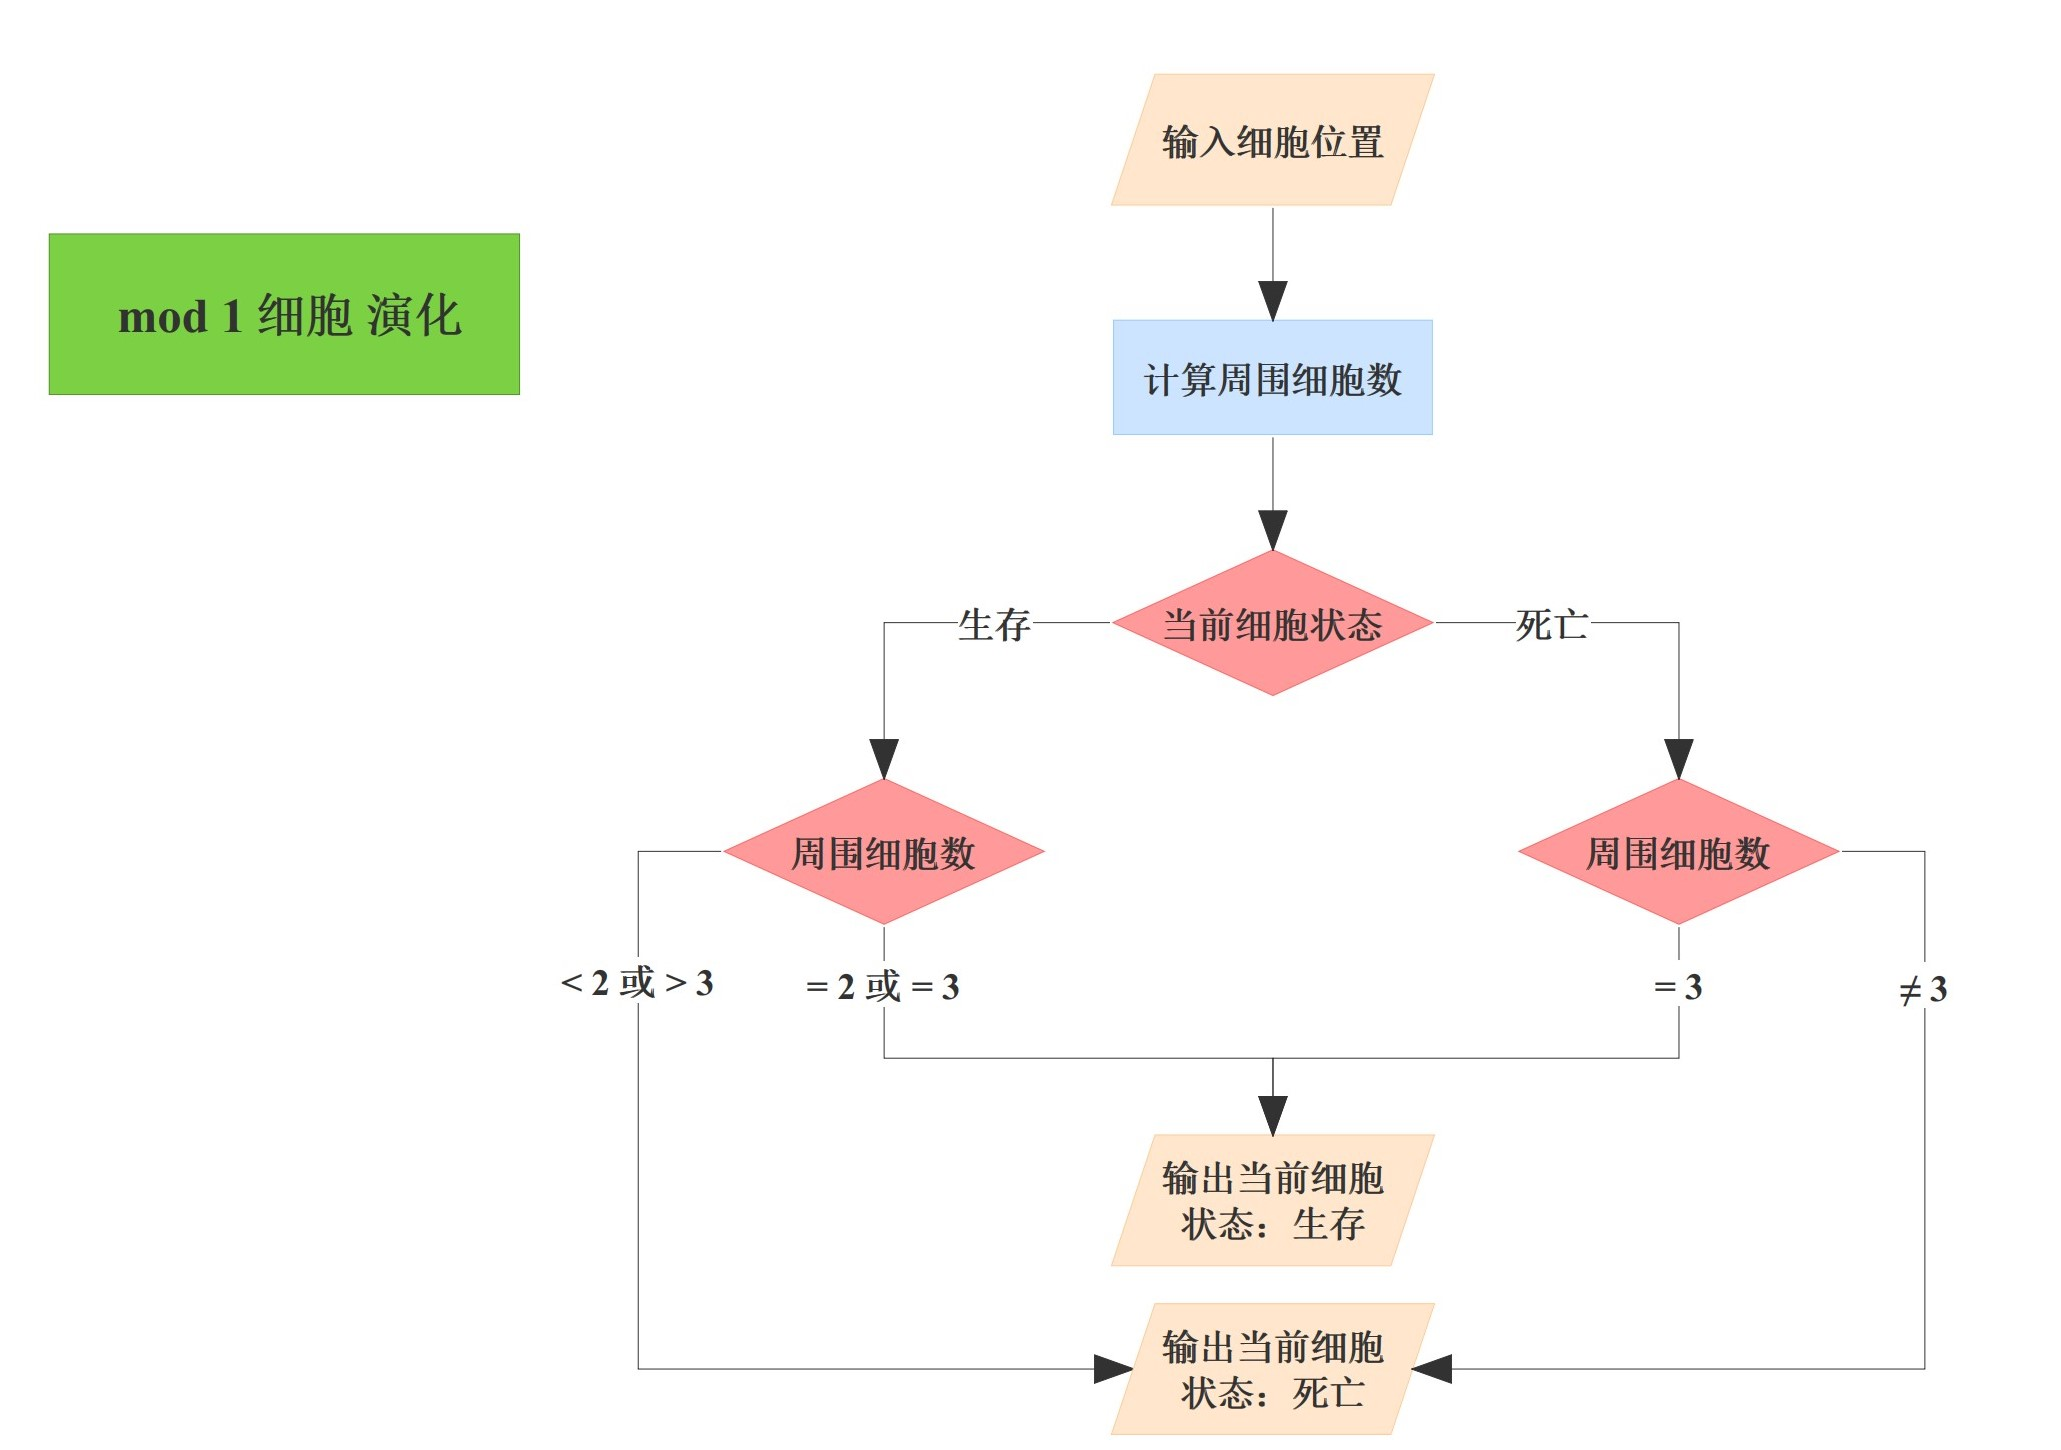
\includegraphics[width = .8\textwidth]{set1/3.jpg}
    \caption{\textbf{mod1 的细胞演化实现}}
\end{figure}
  
\end{itemize}

\hypertarget{mod2ux590dux6742ux6a21ux5f0f}{%
\subsubsection{\texorpdfstring{\texttt{mod2}:复杂模式}{mod2:复杂模式}}\label{mod2ux590dux6742ux6a21ux5f0f}}

\begin{itemize}
\item
  输入实现
\begin{figure}[H]
    \centering
    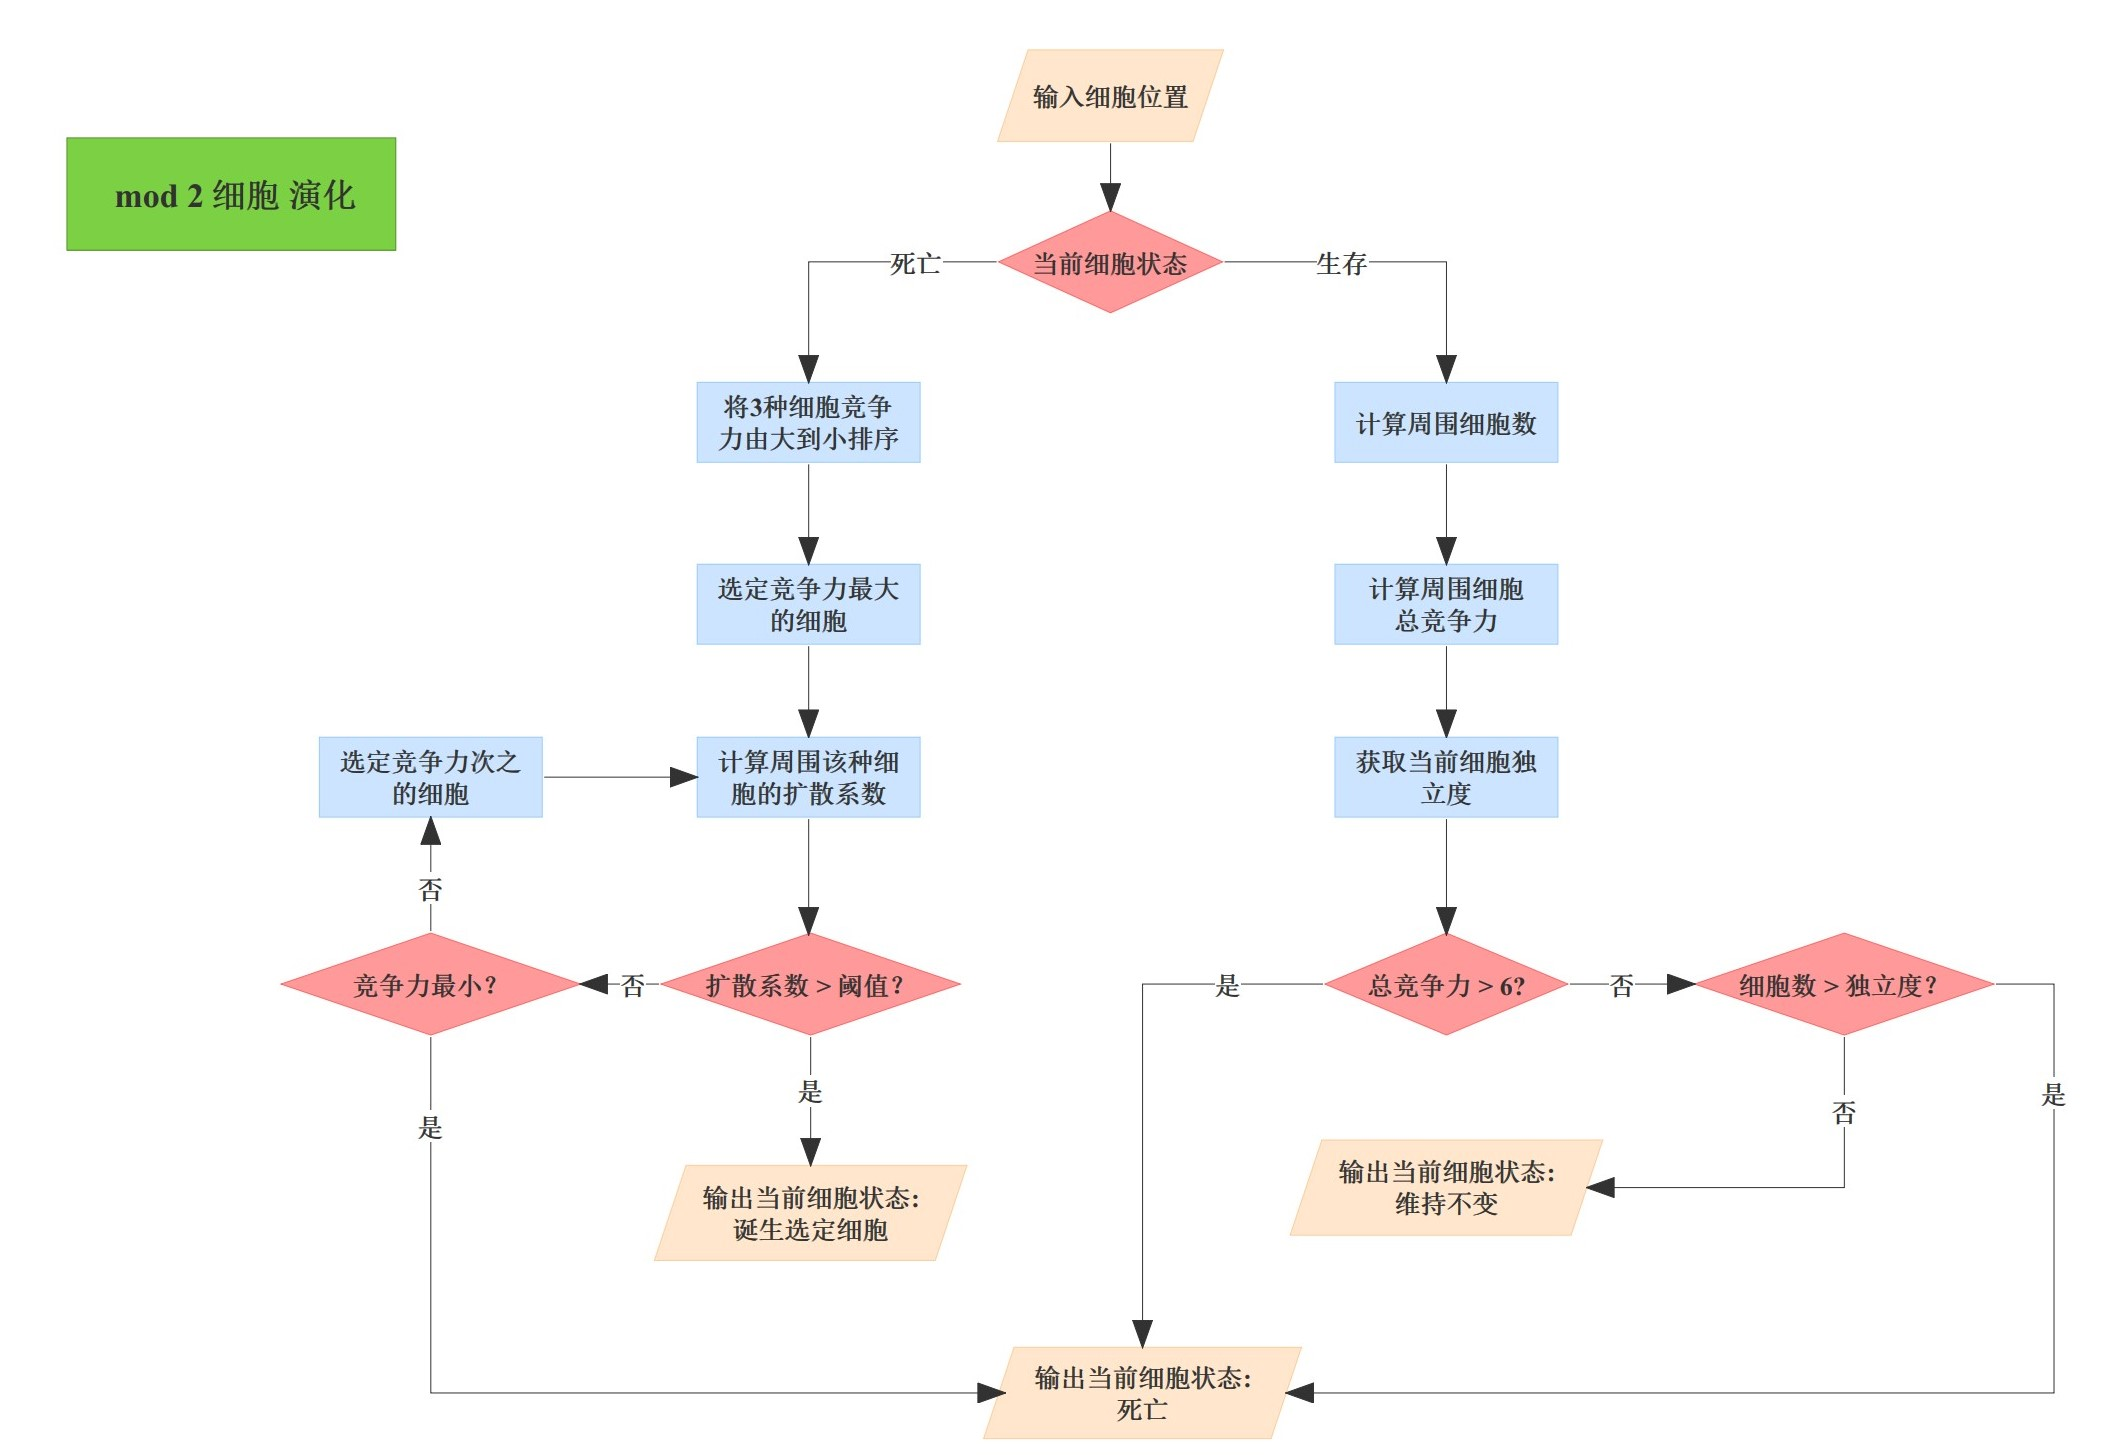
\includegraphics[width = .85\textwidth]{set1/4.jpg}
    \caption{\textbf{mod2 的输入实现}}
\end{figure}
\item
  细胞演化实现
\begin{figure}[H]
    \centering
    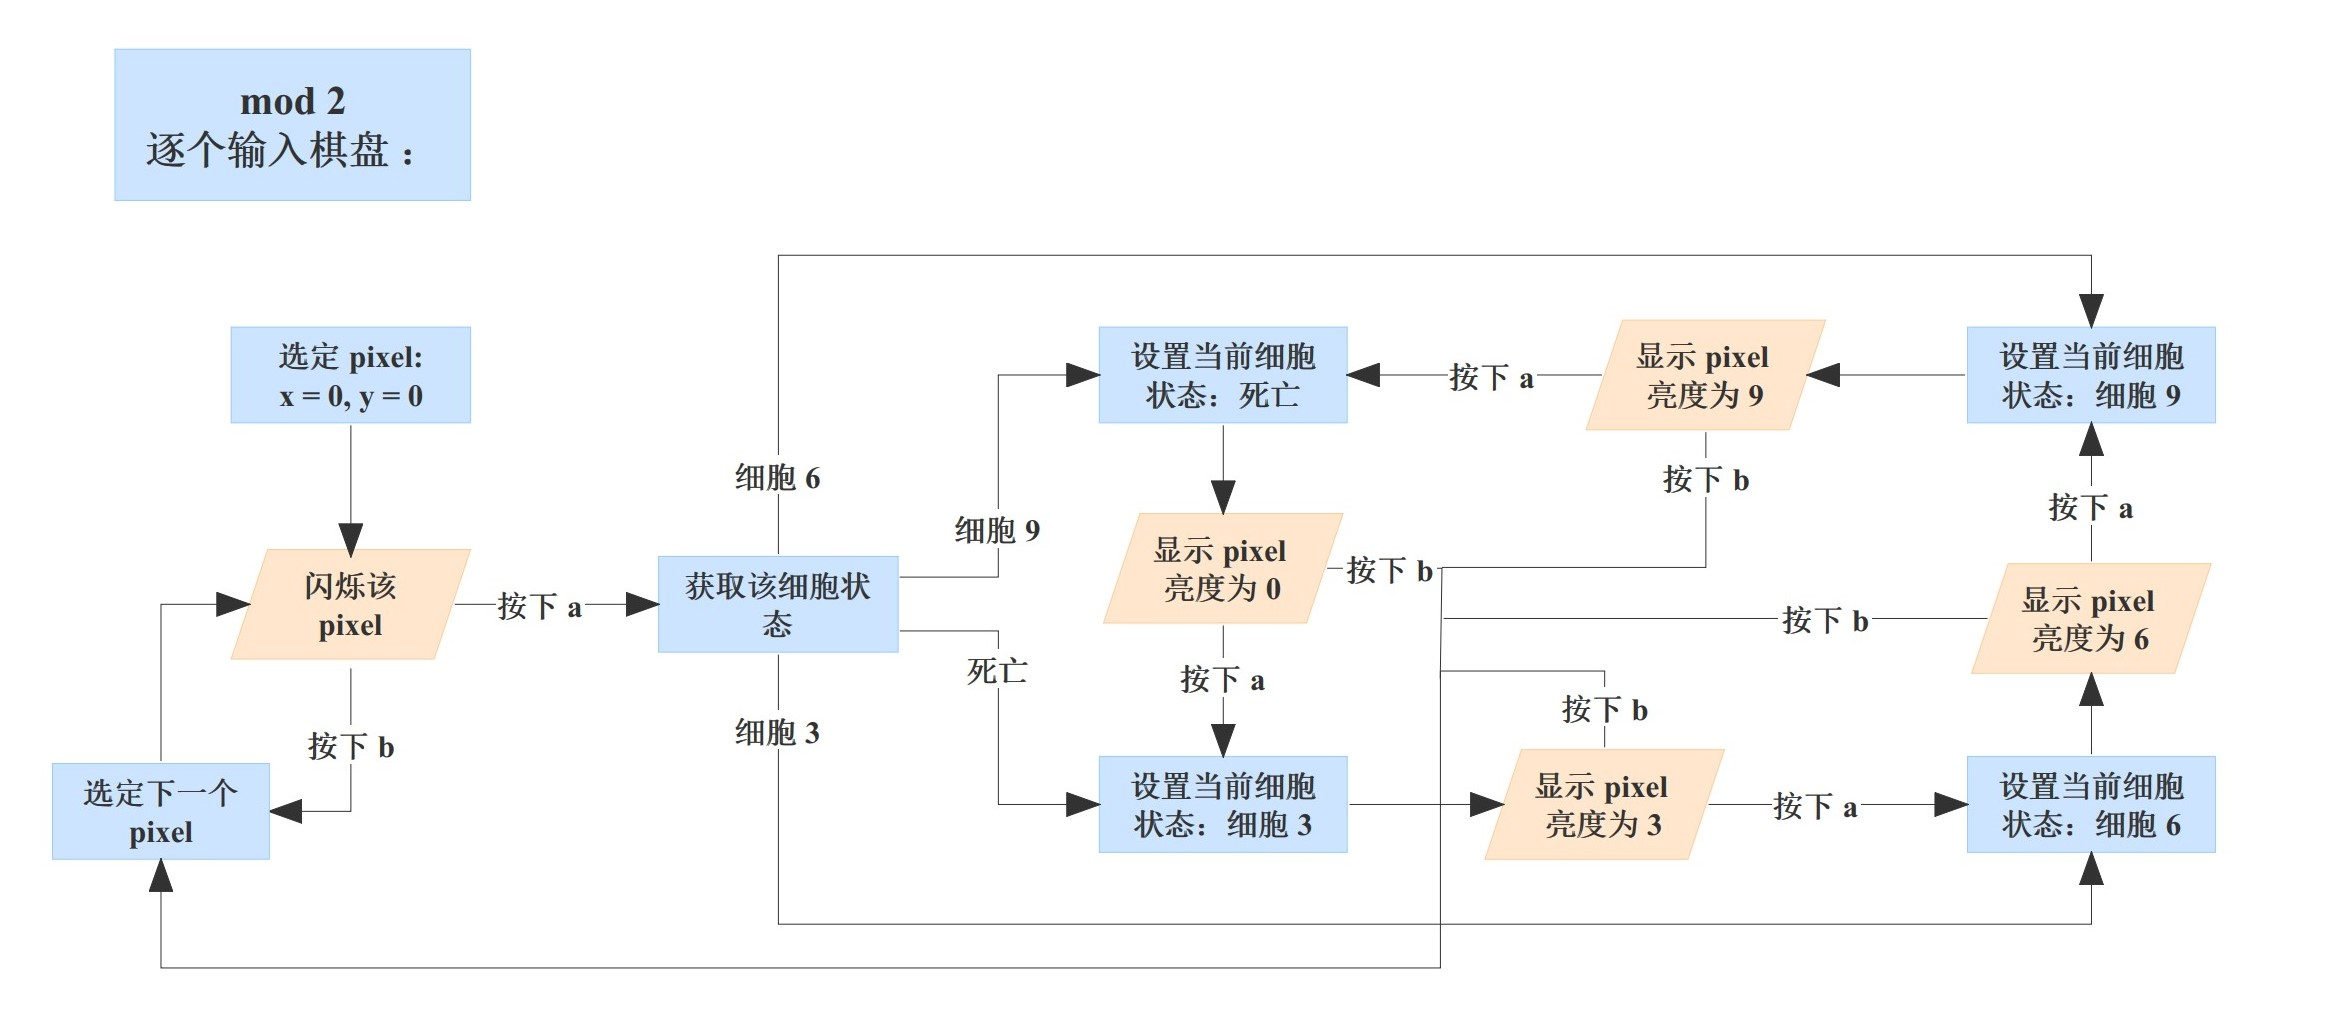
\includegraphics[width = \textwidth]{set1/6.jpg}
    \caption{\textbf{mod2 的细胞演化实现}}
\end{figure}
\end{itemize}

    \hypertarget{ux51fdux6570ux5b9aux4e49}{%
\subsection{函数定义}\label{ux51fdux6570ux5b9aux4e49}}

    \hypertarget{draw_universe-draw_rev_universe-ux4e0e-blink_pixel}{%
\subsubsection{\texorpdfstring{\texttt{draw\_universe} 、
\texttt{draw\_rev\_universe} 与
\texttt{blink\_pixel}}{draw\_universe 、 draw\_rev\_universe 与 blink\_pixel}}\label{draw_universe-draw_rev_universe-ux4e0e-blink_pixel}}

\begin{itemize}
\tightlist
\item
  \texttt{draw\_universe}:用于将棋盘内所有像素点显示
\end{itemize}

    \begin{tcolorbox}[breakable, size=fbox, boxrule=1pt, pad at break*=1mm,colback=cellbackground, colframe=cellborder]
\prompt{In}{incolor}{1}{\boxspacing}
\begin{Verbatim}[commandchars=\\\{\}]
\PY{k}{def} \PY{n+nf}{draw\PYZus{}universe}\PY{p}{(}\PY{n}{universe}\PY{p}{)}\PY{p}{:}
    \PY{k}{for} \PY{n}{y} \PY{o+ow}{in} \PY{n+nb}{range}\PY{p}{(}\PY{l+m+mi}{1}\PY{p}{,} \PY{l+m+mi}{6}\PY{p}{)}\PY{p}{:}
        \PY{k}{for} \PY{n}{x} \PY{o+ow}{in} \PY{n+nb}{range}\PY{p}{(}\PY{l+m+mi}{1}\PY{p}{,} \PY{l+m+mi}{6}\PY{p}{)}\PY{p}{:}
            \PY{n}{display}\PY{o}{.}\PY{n}{set\PYZus{}pixel}\PY{p}{(}\PY{n}{x}\PY{o}{\PYZhy{}}\PY{l+m+mi}{1}\PY{p}{,} \PY{n}{y}\PY{o}{\PYZhy{}}\PY{l+m+mi}{1}\PY{p}{,} \PY{n}{universe}\PY{p}{[}\PY{n}{x} \PY{o}{+} \PY{n}{y} \PY{o}{*} \PY{l+m+mi}{7}\PY{p}{]}\PY{p}{)}
\end{Verbatim}
\end{tcolorbox}

    \begin{itemize}
\tightlist
\item
  \texttt{draw\_rev\_universe}:用于棋盘内除去指定像素点,将其余所有像素点显示,用于\texttt{mod1}和\texttt{mod2}的\texttt{REV}模式
\end{itemize}

    \begin{tcolorbox}[breakable, size=fbox, boxrule=1pt, pad at break*=1mm,colback=cellbackground, colframe=cellborder]
\prompt{In}{incolor}{2}{\boxspacing}
\begin{Verbatim}[commandchars=\\\{\}]
\PY{k}{def} \PY{n+nf}{draw\PYZus{}rev\PYZus{}universe}\PY{p}{(}\PY{n}{universe}\PY{p}{,} \PY{n}{xx}\PY{p}{,} \PY{n}{yy}\PY{p}{)}\PY{p}{:}
    \PY{k}{for} \PY{n}{y} \PY{o+ow}{in} \PY{n+nb}{range}\PY{p}{(}\PY{l+m+mi}{1}\PY{p}{,} \PY{l+m+mi}{6}\PY{p}{)}\PY{p}{:}
        \PY{k}{for} \PY{n}{x} \PY{o+ow}{in} \PY{n+nb}{range}\PY{p}{(}\PY{l+m+mi}{1}\PY{p}{,} \PY{l+m+mi}{6}\PY{p}{)}\PY{p}{:}
            \PY{k}{if} \PY{o+ow}{not} \PY{p}{(}\PY{n}{x} \PY{o}{==} \PY{n}{xx} \PY{o+ow}{and} \PY{n}{y} \PY{o}{==} \PY{n}{yy}\PY{p}{)}\PY{p}{:}
                \PY{n}{display}\PY{o}{.}\PY{n}{set\PYZus{}pixel}\PY{p}{(}\PY{n}{x}\PY{o}{\PYZhy{}}\PY{l+m+mi}{1}\PY{p}{,} \PY{n}{y}\PY{o}{\PYZhy{}}\PY{l+m+mi}{1}\PY{p}{,} \PY{n}{universe}\PY{p}{[}\PY{n}{x} \PY{o}{+} \PY{n}{y} \PY{o}{*} \PY{l+m+mi}{7}\PY{p}{]}\PY{p}{)}
\end{Verbatim}
\end{tcolorbox}

    \begin{itemize}
\tightlist
\item
  \texttt{blink\_pixel}:用于控制指定像素点闪烁一次
\end{itemize}

    \begin{tcolorbox}[breakable, size=fbox, boxrule=1pt, pad at break*=1mm,colback=cellbackground, colframe=cellborder]
\prompt{In}{incolor}{3}{\boxspacing}
\begin{Verbatim}[commandchars=\\\{\}]
\PY{k}{def} \PY{n+nf}{blink\PYZus{}pixel}\PY{p}{(}\PY{n}{x}\PY{p}{,} \PY{n}{y}\PY{p}{)}\PY{p}{:}
    \PY{n}{display}\PY{o}{.}\PY{n}{set\PYZus{}pixel}\PY{p}{(}\PY{n}{x}\PY{p}{,} \PY{n}{y}\PY{p}{,} \PY{l+m+mi}{6}\PY{p}{)}
    \PY{n}{sleep}\PY{p}{(}\PY{l+m+mi}{500}\PY{p}{)}
    \PY{n}{display}\PY{o}{.}\PY{n}{set\PYZus{}pixel}\PY{p}{(}\PY{n}{x}\PY{p}{,} \PY{n}{y}\PY{p}{,} \PY{l+m+mi}{0}\PY{p}{)}
    \PY{n}{sleep}\PY{p}{(}\PY{l+m+mi}{500}\PY{p}{)}
\end{Verbatim}
\end{tcolorbox}

    \hypertarget{evolve_1-ux4e0e-get_neighbours_count}{%
\subsubsection{\texorpdfstring{\texttt{evolve\_1} 与
\texttt{get\_neighbours\_count}}{evolve\_1 与 get\_neighbours\_count}}\label{evolve_1-ux4e0e-get_neighbours_count}}

\begin{itemize}
\tightlist
\item
  \texttt{evlove\_1}:用于\texttt{mod1}中的演化

  \begin{itemize}
  \tightlist
  \item
    使用\texttt{get\_neighbours\_count}计算周围细胞数
  \item
    若细胞状态为生存:

    \begin{itemize}
    \tightlist
    \item
      周围细胞数为2或3,保持生存
    \item
      周围细胞数小于2或大于3,死亡
    \end{itemize}
  \item
    若细胞状态为死亡:

    \begin{itemize}
    \tightlist
    \item
      周围细胞数等于3,诞生细胞
    \item
      周围细胞数不等于3,保持死亡
    \end{itemize}
  \end{itemize}
\end{itemize}

    \begin{tcolorbox}[breakable, size=fbox, boxrule=1pt, pad at break*=1mm,colback=cellbackground, colframe=cellborder]
\prompt{In}{incolor}{4}{\boxspacing}
\begin{Verbatim}[commandchars=\\\{\}]
\PY{k}{def} \PY{n+nf}{evolve\PYZus{}1}\PY{p}{(}\PY{n}{universe}\PY{p}{)}\PY{p}{:}
    \PY{n}{next\PYZus{}universe} \PY{o}{=} \PY{n}{universe}\PY{p}{[}\PY{p}{:}\PY{p}{]}
    \PY{k}{for} \PY{n}{y} \PY{o+ow}{in} \PY{n+nb}{range}\PY{p}{(}\PY{l+m+mi}{1}\PY{p}{,} \PY{l+m+mi}{6}\PY{p}{)}\PY{p}{:}
        \PY{k}{for} \PY{n}{x} \PY{o+ow}{in} \PY{n+nb}{range}\PY{p}{(}\PY{l+m+mi}{1}\PY{p}{,} \PY{l+m+mi}{6}\PY{p}{)}\PY{p}{:}
            \PY{n}{count\PYZus{}neighbours} \PY{o}{=} \PY{n}{get\PYZus{}neighbours\PYZus{}count}\PY{p}{(}\PY{n}{universe}\PY{p}{,} \PY{n}{x}\PY{p}{,} \PY{n}{y}\PY{p}{)}
            \PY{k}{if} \PY{o+ow}{not} \PY{n}{universe}\PY{p}{[}\PY{n}{x} \PY{o}{+} \PY{l+m+mi}{7} \PY{o}{*} \PY{n}{y}\PY{p}{]}\PY{p}{:}
                \PY{k}{if} \PY{n}{count\PYZus{}neighbours} \PY{o}{==} \PY{l+m+mi}{3}\PY{p}{:}
                    \PY{n}{next\PYZus{}universe}\PY{p}{[}\PY{n}{x} \PY{o}{+} \PY{l+m+mi}{7} \PY{o}{*} \PY{n}{y}\PY{p}{]} \PY{o}{=} \PY{l+m+mi}{9}   \PY{c+c1}{\PYZsh{} 新生命的诞生}
            \PY{k}{else}\PY{p}{:}
                \PY{k}{if} \PY{n}{count\PYZus{}neighbours} \PY{o}{\PYZlt{}} \PY{l+m+mi}{2}\PY{p}{:}
                    \PY{n}{next\PYZus{}universe}\PY{p}{[}\PY{n}{x} \PY{o}{+} \PY{l+m+mi}{7} \PY{o}{*} \PY{n}{y}\PY{p}{]} \PY{o}{=} \PY{l+m+mi}{0}  \PY{c+c1}{\PYZsh{} 生命因孤独而死亡}
                \PY{k}{elif} \PY{n}{count\PYZus{}neighbours} \PY{o}{\PYZgt{}} \PY{l+m+mi}{3}\PY{p}{:}
                    \PY{n}{next\PYZus{}universe}\PY{p}{[}\PY{n}{x} \PY{o}{+} \PY{l+m+mi}{7} \PY{o}{*} \PY{n}{y}\PY{p}{]} \PY{o}{=} \PY{l+m+mi}{0}  \PY{c+c1}{\PYZsh{} 生命因拥挤而死亡}
                \PY{k}{else}\PY{p}{:}
                    \PY{k}{pass}

    \PY{k}{return} \PY{n}{next\PYZus{}universe}
\end{Verbatim}
\end{tcolorbox}

    \begin{itemize}
\tightlist
\item
  \texttt{get\_neighbours\_count}:用于计算指定细胞周围,状态为生存的总细胞数
\end{itemize}

    \begin{tcolorbox}[breakable, size=fbox, boxrule=1pt, pad at break*=1mm,colback=cellbackground, colframe=cellborder]
\prompt{In}{incolor}{5}{\boxspacing}
\begin{Verbatim}[commandchars=\\\{\}]
\PY{k}{def} \PY{n+nf}{get\PYZus{}neighbours\PYZus{}count}\PY{p}{(}\PY{n}{universe}\PY{p}{,} \PY{n}{x}\PY{p}{,} \PY{n}{y}\PY{p}{)}\PY{p}{:}
    \PY{n}{count\PYZus{}neighbours} \PY{o}{=} \PY{l+m+mi}{0}
    \PY{k}{for} \PY{n}{dy} \PY{o+ow}{in} \PY{p}{[}\PY{o}{\PYZhy{}}\PY{l+m+mi}{1}\PY{p}{,} \PY{l+m+mi}{0}\PY{p}{,} \PY{l+m+mi}{1}\PY{p}{]}\PY{p}{:} 
        \PY{k}{for} \PY{n}{dx} \PY{o+ow}{in} \PY{p}{[}\PY{o}{\PYZhy{}}\PY{l+m+mi}{1}\PY{p}{,} \PY{l+m+mi}{0}\PY{p}{,} \PY{l+m+mi}{1}\PY{p}{]}\PY{p}{:}
            \PY{k}{if} \PY{n}{dx} \PY{o}{==} \PY{l+m+mi}{0} \PY{o+ow}{and} \PY{n}{dy} \PY{o}{==} \PY{l+m+mi}{0}\PY{p}{:}
                \PY{k}{pass}
            \PY{k}{elif} \PY{n}{universe}\PY{p}{[}\PY{p}{(}\PY{n}{x} \PY{o}{+} \PY{n}{dx}\PY{p}{)} \PY{o}{+} \PY{l+m+mi}{7} \PY{o}{*} \PY{p}{(}\PY{n}{y} \PY{o}{+} \PY{n}{dy}\PY{p}{)}\PY{p}{]} \PY{o}{==} \PY{l+m+mi}{0}\PY{p}{:}
                \PY{k}{pass}
            \PY{k}{else}\PY{p}{:}
                \PY{n}{count\PYZus{}neighbours} \PY{o}{+}\PY{o}{=} \PY{l+m+mi}{1}    
    \PY{k}{return} \PY{n}{count\PYZus{}neighbours}
\end{Verbatim}
\end{tcolorbox}

    \hypertarget{evolve_1-get_neighbours_diff-ux4e0e-get_neighbours_cc}{%
\subsubsection{\texorpdfstring{\texttt{evolve\_1} 、
\texttt{get\_neighbours\_diff} 与
\texttt{get\_neighbours\_cc}}{evolve\_1 、 get\_neighbours\_diff 与 get\_neighbours\_cc}}\label{evolve_1-get_neighbours_diff-ux4e0e-get_neighbours_cc}}

\begin{itemize}
\tightlist
\item
  \texttt{evlove\_2}:用于\texttt{mod2}中的演化

  \begin{itemize}
  \tightlist
  \item
    若细胞状态为死亡

    \begin{itemize}
    \tightlist
    \item
      使用\texttt{get\_neighbours\_diff}返回细胞演化后的状态
    \end{itemize}
  \item
    若细胞状态为生存

    \begin{itemize}
    \tightlist
    \item
      使用\texttt{get\_neighbours\_cc}返回细胞周围的总细胞数与总竞争度

      \begin{itemize}
      \tightlist
      \item
        若总细胞数小于细胞独立度\texttt{dependence},细胞因孤独而死
      \item
        若总竞争度大于等于6,细胞因拥挤而死
      \end{itemize}
    \end{itemize}
  \end{itemize}
\end{itemize}

    \begin{tcolorbox}[breakable, size=fbox, boxrule=1pt, pad at break*=1mm,colback=cellbackground, colframe=cellborder]
\prompt{In}{incolor}{6}{\boxspacing}
\begin{Verbatim}[commandchars=\\\{\}]
\PY{k}{def} \PY{n+nf}{evolve\PYZus{}2}\PY{p}{(}\PY{n}{universe}\PY{p}{)}\PY{p}{:}
    \PY{n}{next\PYZus{}universe} \PY{o}{=} \PY{n}{universe}\PY{p}{[}\PY{p}{:}\PY{p}{]}
    \PY{k}{for} \PY{n}{y} \PY{o+ow}{in} \PY{n+nb}{range}\PY{p}{(}\PY{l+m+mi}{1}\PY{p}{,} \PY{l+m+mi}{6}\PY{p}{)}\PY{p}{:}
        \PY{k}{for} \PY{n}{x} \PY{o+ow}{in} \PY{n+nb}{range}\PY{p}{(}\PY{l+m+mi}{1}\PY{p}{,} \PY{l+m+mi}{6}\PY{p}{)}\PY{p}{:}
            \PY{k}{if} \PY{o+ow}{not} \PY{n}{universe}\PY{p}{[}\PY{n}{x} \PY{o}{+} \PY{l+m+mi}{7} \PY{o}{*} \PY{n}{y}\PY{p}{]}\PY{p}{:}
                \PY{n}{next\PYZus{}universe}\PY{p}{[}\PY{n}{x} \PY{o}{+} \PY{l+m+mi}{7} \PY{o}{*} \PY{n}{y}\PY{p}{]} \PY{o}{=} \PY{n}{get\PYZus{}neighbours\PYZus{}diff}\PY{p}{(}\PY{n}{universe}\PY{p}{,} \PY{n}{x}\PY{p}{,} \PY{n}{y}\PY{p}{)}  \PY{c+c1}{\PYZsh{} 新生命的诞生}
            \PY{k}{else}\PY{p}{:}
                \PY{n}{count\PYZus{}neighbours}\PY{p}{,} \PY{n}{compet\PYZus{}neighbours} \PY{o}{=} \PY{n}{get\PYZus{}neighbours\PYZus{}cc}\PY{p}{(}\PY{n}{universe}\PY{p}{,} \PY{n}{x}\PY{p}{,} \PY{n}{y}\PY{p}{)}
                \PY{k}{if} \PY{n}{count\PYZus{}neighbours} \PY{o}{\PYZlt{}} \PY{n}{dependence}\PY{p}{[}\PY{n}{universe}\PY{p}{[}\PY{n}{x}\PY{o}{+}\PY{l+m+mi}{7}\PY{o}{*}\PY{n}{y}\PY{p}{]}\PY{p}{]}\PY{p}{:}
                    \PY{n}{next\PYZus{}universe}\PY{p}{[}\PY{n}{x} \PY{o}{+} \PY{l+m+mi}{7} \PY{o}{*} \PY{n}{y}\PY{p}{]} \PY{o}{=} \PY{l+m+mi}{0}  \PY{c+c1}{\PYZsh{} 生命因孤独而死亡}
                \PY{k}{elif} \PY{n}{compet\PYZus{}neighbours} \PY{o}{\PYZgt{}}\PY{o}{=} \PY{l+m+mi}{6}\PY{p}{:}
                    \PY{n}{next\PYZus{}universe}\PY{p}{[}\PY{n}{x} \PY{o}{+} \PY{l+m+mi}{7} \PY{o}{*} \PY{n}{y}\PY{p}{]} \PY{o}{=} \PY{l+m+mi}{0}  \PY{c+c1}{\PYZsh{} 生命因拥挤而死亡}
                \PY{k}{else}\PY{p}{:}
                    \PY{k}{pass}

    \PY{k}{return} \PY{n}{next\PYZus{}universe}
\end{Verbatim}
\end{tcolorbox}

    \begin{itemize}
\tightlist
\item
  \texttt{get\_neighbours\_diff}:用于根据扩散系数\texttt{diffusion}计算细胞扩散结果

  \begin{itemize}
  \tightlist
  \item
    将三种细胞(3,6,9)按照竞争力\texttt{competitiveness}排序
  \item
    按竞争力从大到小的顺序,依次选定该种细胞
  \item
    计算当前细胞周围的细胞中,该种细胞的总个数
  \item
    若该种细胞总个数大于该种细胞独立度\texttt{dependence},诞生新的该种细胞
  \item
    若小于独立度,选定竞争力次之的细胞,重复上述过程
  \item
    若始终无法大于独立度,则保持死亡状态
  \end{itemize}
\end{itemize}

    \begin{tcolorbox}[breakable, size=fbox, boxrule=1pt, pad at break*=1mm,colback=cellbackground, colframe=cellborder]
\prompt{In}{incolor}{7}{\boxspacing}
\begin{Verbatim}[commandchars=\\\{\}]
\PY{k}{def} \PY{n+nf}{get\PYZus{}neighbours\PYZus{}diff}\PY{p}{(}\PY{n}{universe}\PY{p}{,} \PY{n}{x}\PY{p}{,} \PY{n}{y}\PY{p}{)}\PY{p}{:}
    \PY{n}{compet\PYZus{}values} \PY{o}{=} \PY{p}{[}\PY{n}{value} \PY{k}{for} \PY{n}{value} \PY{o+ow}{in} \PY{n}{competitiveness}\PY{o}{.}\PY{n}{values}\PY{p}{(}\PY{p}{)}\PY{p}{]}
    \PY{n}{compet\PYZus{}values}\PY{o}{.}\PY{n}{sort}\PY{p}{(}\PY{n}{reverse} \PY{o}{=} \PY{k+kc}{True}\PY{p}{)}
    \PY{k}{for} \PY{n}{value} \PY{o+ow}{in} \PY{n}{compet\PYZus{}values}\PY{p}{:}
        \PY{n}{key} \PY{o}{=} \PY{n}{reverse\PYZus{}competitiveness}\PY{p}{[}\PY{n}{value}\PY{p}{]}
        \PY{n}{diff\PYZus{}count} \PY{o}{=} \PY{l+m+mi}{0}
        \PY{k}{for} \PY{n}{dy} \PY{o+ow}{in} \PY{p}{[}\PY{o}{\PYZhy{}}\PY{l+m+mi}{1}\PY{p}{,} \PY{l+m+mi}{0}\PY{p}{,} \PY{l+m+mi}{1}\PY{p}{]}\PY{p}{:}
            \PY{k}{for} \PY{n}{dx} \PY{o+ow}{in} \PY{p}{[}\PY{o}{\PYZhy{}}\PY{l+m+mi}{1}\PY{p}{,} \PY{l+m+mi}{0}\PY{p}{,} \PY{l+m+mi}{1}\PY{p}{]}\PY{p}{:}
                \PY{k}{if} \PY{n}{dx} \PY{o}{==} \PY{l+m+mi}{0} \PY{o+ow}{and} \PY{n}{dy} \PY{o}{==} \PY{l+m+mi}{0}\PY{p}{:}
                    \PY{k}{pass}
                \PY{k}{elif} \PY{o+ow}{not} \PY{n}{universe}\PY{p}{[}\PY{p}{(}\PY{n}{x} \PY{o}{+} \PY{n}{dx}\PY{p}{)} \PY{o}{+} \PY{l+m+mi}{7} \PY{o}{*} \PY{p}{(}\PY{n}{y} \PY{o}{+} \PY{n}{dy}\PY{p}{)}\PY{p}{]}\PY{p}{:}
                    \PY{k}{pass}
                \PY{k}{elif} \PY{n}{universe}\PY{p}{[}\PY{p}{(}\PY{n}{x} \PY{o}{+} \PY{n}{dx}\PY{p}{)} \PY{o}{+} \PY{l+m+mi}{7} \PY{o}{*} \PY{p}{(}\PY{n}{y} \PY{o}{+} \PY{n}{dy}\PY{p}{)}\PY{p}{]} \PY{o}{==} \PY{n}{key}\PY{p}{:}
                    \PY{n}{diff\PYZus{}count} \PY{o}{+}\PY{o}{=} \PY{l+m+mi}{1}
                \PY{k}{else}\PY{p}{:}
                    \PY{k}{pass}
        \PY{k}{if} \PY{n}{diff\PYZus{}count} \PY{o}{\PYZgt{}}\PY{o}{=} \PY{n}{diffusion}\PY{p}{[}\PY{n}{key}\PY{p}{]}\PY{p}{:}
            \PY{k}{return} \PY{n}{key}
    \PY{k}{return} \PY{l+m+mi}{0}
\end{Verbatim}
\end{tcolorbox}

    \begin{itemize}
\tightlist
\item
  \texttt{get\_neighbours\_cc}:用于返回指定细胞周围,状态为生存的总细胞数,并根据对应细胞竞争力\texttt{competitiveness}的和返回总竞争度
\end{itemize}

    \begin{tcolorbox}[breakable, size=fbox, boxrule=1pt, pad at break*=1mm,colback=cellbackground, colframe=cellborder]
\prompt{In}{incolor}{8}{\boxspacing}
\begin{Verbatim}[commandchars=\\\{\}]
\PY{k}{def} \PY{n+nf}{get\PYZus{}neighbours\PYZus{}cc}\PY{p}{(}\PY{n}{universe}\PY{p}{,} \PY{n}{x}\PY{p}{,} \PY{n}{y}\PY{p}{)}\PY{p}{:}
    \PY{n}{count\PYZus{}neighbours}\PY{p}{,} \PY{n}{compet\PYZus{}neighbours} \PY{o}{=} \PY{l+m+mi}{0}\PY{p}{,} \PY{l+m+mi}{0}
    \PY{k}{for} \PY{n}{dy} \PY{o+ow}{in} \PY{p}{[}\PY{o}{\PYZhy{}}\PY{l+m+mi}{1}\PY{p}{,} \PY{l+m+mi}{0}\PY{p}{,} \PY{l+m+mi}{1}\PY{p}{]}\PY{p}{:}
        \PY{k}{for} \PY{n}{dx} \PY{o+ow}{in} \PY{p}{[}\PY{o}{\PYZhy{}}\PY{l+m+mi}{1}\PY{p}{,} \PY{l+m+mi}{0}\PY{p}{,} \PY{l+m+mi}{1}\PY{p}{]}\PY{p}{:}
            \PY{k}{if} \PY{n}{dx} \PY{o}{==} \PY{l+m+mi}{0} \PY{o+ow}{and} \PY{n}{dy} \PY{o}{==} \PY{l+m+mi}{0}\PY{p}{:}
                \PY{k}{pass}
            \PY{k}{elif} \PY{o+ow}{not} \PY{n}{universe}\PY{p}{[}\PY{p}{(}\PY{n}{x} \PY{o}{+} \PY{n}{dx}\PY{p}{)} \PY{o}{+} \PY{l+m+mi}{7} \PY{o}{*} \PY{p}{(}\PY{n}{y} \PY{o}{+} \PY{n}{dy}\PY{p}{)}\PY{p}{]}\PY{p}{:}
                \PY{k}{pass}
            \PY{k}{else}\PY{p}{:}
                \PY{n}{cur} \PY{o}{=} \PY{n}{universe}\PY{p}{[}\PY{p}{(}\PY{n}{x} \PY{o}{+} \PY{n}{dx}\PY{p}{)} \PY{o}{+} \PY{l+m+mi}{7} \PY{o}{*} \PY{p}{(}\PY{n}{y} \PY{o}{+} \PY{n}{dy}\PY{p}{)}\PY{p}{]}
                \PY{n}{count\PYZus{}neighbours} \PY{o}{+}\PY{o}{=} \PY{n}{cur} \PY{o}{/}\PY{o}{/} \PY{l+m+mi}{3}
                \PY{n}{compet\PYZus{}neighbours} \PY{o}{+}\PY{o}{=} \PY{n}{competitiveness}\PY{p}{[}\PY{n}{cur}\PY{p}{]}
    \PY{k}{return} \PY{n}{count\PYZus{}neighbours}\PY{p}{,} \PY{n}{compet\PYZus{}neighbours}
\end{Verbatim}
\end{tcolorbox}

    \hypertarget{pixel_set_1-ux4e0e-pixel_set_2}{%
\subsubsection{\texorpdfstring{\texttt{pixel\_set\_1} 与
\texttt{pixel\_set\_2}}{pixel\_set\_1 与 pixel\_set\_2}}\label{pixel_set_1-ux4e0e-pixel_set_2}}

\begin{itemize}
\tightlist
\item
  \texttt{pixel\_set\_1}:用于在\texttt{mod1}中设置指定像细胞(像素点)的状态

  \begin{itemize}
  \tightlist
  \item
    若无任何操作,待设置状态的细胞对应像素点闪烁
  \item
    每按下一次a键,更新一次状态,使之与之前状态不同,规则如下:

    \begin{itemize}
    \tightlist
    \item
      若之前状态为死亡,更新后状态为生存
    \item
      若之前状态为生存,更新后状态为死亡
    \end{itemize}
  \item
    在中途任意时刻按下b键,固定当前细胞的状态,进入下一个细胞的编辑中
  \item
    在中途任意时刻遮挡感光元件,固定之前设置的所有状态,直接跳入\texttt{RUN}模式中,这样可以节省大量设置时间
  \end{itemize}
\end{itemize}

    \begin{tcolorbox}[breakable, size=fbox, boxrule=1pt, pad at break*=1mm,colback=cellbackground, colframe=cellborder]
\prompt{In}{incolor}{9}{\boxspacing}
\begin{Verbatim}[commandchars=\\\{\}]
\PY{k}{def} \PY{n+nf}{pixel\PYZus{}set\PYZus{}1}\PY{p}{(}\PY{n}{x}\PY{p}{,} \PY{n}{y}\PY{p}{,} \PY{n}{light}\PY{p}{)}\PY{p}{:}
    \PY{k}{while} \PY{o+ow}{not} \PY{n}{button\PYZus{}a}\PY{o}{.}\PY{n}{is\PYZus{}pressed}\PY{p}{(}\PY{p}{)}\PY{p}{:}
        \PY{n}{blink\PYZus{}pixel}\PY{p}{(}\PY{n}{x}\PY{o}{\PYZhy{}}\PY{l+m+mi}{1}\PY{p}{,} \PY{n}{y}\PY{o}{\PYZhy{}}\PY{l+m+mi}{1}\PY{p}{)}
        \PY{n}{light} \PY{o}{=} \PY{p}{(}\PY{n}{display}\PY{o}{.}\PY{n}{read\PYZus{}light\PYZus{}level}\PY{p}{(}\PY{p}{)} \PY{o}{\PYZlt{}} \PY{l+m+mi}{30}\PY{p}{)}
        \PY{k}{if} \PY{n}{button\PYZus{}b}\PY{o}{.}\PY{n}{is\PYZus{}pressed}\PY{p}{(}\PY{p}{)} \PY{o+ow}{or} \PY{n}{light}\PY{p}{:}
            \PY{k}{break}
    \PY{k}{else}\PY{p}{:}
        \PY{n}{is\PYZus{}pressed\PYZus{}a} \PY{o}{=} \PY{k+kc}{True}
        \PY{n}{sleep}\PY{p}{(}\PY{l+m+mi}{500}\PY{p}{)}
        \PY{k}{while} \PY{n}{is\PYZus{}pressed\PYZus{}a}\PY{p}{:}
            \PY{n}{cur} \PY{o}{=} \PY{n}{current\PYZus{}universe}\PY{p}{[}\PY{n}{x} \PY{o}{+} \PY{l+m+mi}{7} \PY{o}{*} \PY{n}{y}\PY{p}{]}
            \PY{n}{current\PYZus{}universe}\PY{p}{[}\PY{n}{x} \PY{o}{+} \PY{l+m+mi}{7} \PY{o}{*} \PY{n}{y}\PY{p}{]} \PY{o}{=} \PY{l+m+mi}{9} \PY{k}{if} \PY{n}{cur} \PY{o}{==} \PY{l+m+mi}{0} \PY{k}{else} \PY{l+m+mi}{0} \PY{k}{if} \PY{n}{cur} \PY{o}{==} \PY{l+m+mi}{9} \PY{k}{else} \PY{n}{cur}     \PY{c+c1}{\PYZsh{} 循环设置 0 与 9}
            \PY{n}{display}\PY{o}{.}\PY{n}{set\PYZus{}pixel}\PY{p}{(}\PY{n}{x}\PY{o}{\PYZhy{}}\PY{l+m+mi}{1}\PY{p}{,} \PY{n}{y}\PY{o}{\PYZhy{}}\PY{l+m+mi}{1}\PY{p}{,} \PY{n}{current\PYZus{}universe}\PY{p}{[}\PY{n}{x} \PY{o}{+} \PY{l+m+mi}{7} \PY{o}{*} \PY{n}{y}\PY{p}{]}\PY{p}{)}
            \PY{n}{sleep}\PY{p}{(}\PY{l+m+mi}{500}\PY{p}{)}
            \PY{k}{while} \PY{k+kc}{True}\PY{p}{:}
                \PY{n}{light} \PY{o}{=} \PY{p}{(}\PY{n}{display}\PY{o}{.}\PY{n}{read\PYZus{}light\PYZus{}level}\PY{p}{(}\PY{p}{)} \PY{o}{\PYZlt{}} \PY{l+m+mi}{30}\PY{p}{)}       \PY{c+c1}{\PYZsh{} 通过光线传感器来判断是否需要退出}
                \PY{k}{if} \PY{n}{button\PYZus{}b}\PY{o}{.}\PY{n}{is\PYZus{}pressed}\PY{p}{(}\PY{p}{)} \PY{o+ow}{or} \PY{n}{light}\PY{p}{:}
                    \PY{n}{is\PYZus{}pressed\PYZus{}a} \PY{o}{=} \PY{k+kc}{False}
                    \PY{n}{sleep}\PY{p}{(}\PY{l+m+mi}{500}\PY{p}{)}
                    \PY{k}{break}
                \PY{k}{if} \PY{n}{button\PYZus{}a}\PY{o}{.}\PY{n}{is\PYZus{}pressed}\PY{p}{(}\PY{p}{)}\PY{p}{:}
                    \PY{n}{is\PYZus{}pressed\PYZus{}a} \PY{o}{=} \PY{k+kc}{True}
                    \PY{n}{sleep}\PY{p}{(}\PY{l+m+mi}{500}\PY{p}{)}
                    \PY{k}{break}
    \PY{k}{return} \PY{n}{light}
\end{Verbatim}
\end{tcolorbox}

    \begin{itemize}
\tightlist
\item
  \texttt{pixel\_set\_1}:用于在\texttt{mod1}中设置指定像细胞(像素点)的状态

  \begin{itemize}
  \tightlist
  \item
    若无任何操作,待设置状态的细胞对应像素点闪烁
  \item
    每按下一次a键,更新一次状态,使之与之前状态不同,规则如下:

    \begin{itemize}
    \tightlist
    \item
      若之前状态为死亡,更新后状态为细胞 3
    \item
      若之前状态为细胞 3,更新后状态为细胞 6
    \item
      若之前状态为细胞 6,更新后状态为细胞 9
    \item
      若之前状态为细胞 9,更新后状态为死亡
    \end{itemize}
  \item
    在中途任意时刻按下b键,固定当前细胞的状态,进入下一个细胞的编辑中
  \item
    在中途任意时刻遮挡感光元件,固定之前设置的所有状态,直接结束设置,这样可以节省大量设置时间
  \end{itemize}
\end{itemize}

    \begin{tcolorbox}[breakable, size=fbox, boxrule=1pt, pad at break*=1mm,colback=cellbackground, colframe=cellborder]
\prompt{In}{incolor}{10}{\boxspacing}
\begin{Verbatim}[commandchars=\\\{\}]
\PY{k}{def} \PY{n+nf}{pixel\PYZus{}set\PYZus{}2}\PY{p}{(}\PY{n}{x}\PY{p}{,} \PY{n}{y}\PY{p}{,} \PY{n}{light}\PY{p}{)}\PY{p}{:}
    \PY{k}{while} \PY{o+ow}{not} \PY{n}{button\PYZus{}a}\PY{o}{.}\PY{n}{is\PYZus{}pressed}\PY{p}{(}\PY{p}{)}\PY{p}{:}
        \PY{n}{blink\PYZus{}pixel}\PY{p}{(}\PY{n}{x}\PY{o}{\PYZhy{}}\PY{l+m+mi}{1}\PY{p}{,} \PY{n}{y}\PY{o}{\PYZhy{}}\PY{l+m+mi}{1}\PY{p}{)}
        \PY{n}{light} \PY{o}{=} \PY{p}{(}\PY{n}{display}\PY{o}{.}\PY{n}{read\PYZus{}light\PYZus{}level}\PY{p}{(}\PY{p}{)} \PY{o}{\PYZlt{}} \PY{l+m+mi}{30}\PY{p}{)}
        \PY{k}{if} \PY{n}{button\PYZus{}b}\PY{o}{.}\PY{n}{is\PYZus{}pressed}\PY{p}{(}\PY{p}{)} \PY{o+ow}{or} \PY{n}{light}\PY{p}{:}
            \PY{k}{break}
    \PY{k}{else}\PY{p}{:}
        \PY{n}{is\PYZus{}pressed\PYZus{}a} \PY{o}{=} \PY{k+kc}{True}
        \PY{n}{sleep}\PY{p}{(}\PY{l+m+mi}{500}\PY{p}{)}
        \PY{n}{press\PYZus{}a\PYZus{}count} \PY{o}{=} \PY{l+m+mi}{1}       
        \PY{k}{while} \PY{n}{is\PYZus{}pressed\PYZus{}a}\PY{p}{:}
            \PY{n}{press\PYZus{}a\PYZus{}count} \PY{o}{\PYZpc{}}\PY{o}{=} \PY{l+m+mi}{4}
            \PY{n}{current\PYZus{}universe}\PY{p}{[}\PY{n}{x} \PY{o}{+} \PY{l+m+mi}{7} \PY{o}{*} \PY{n}{y}\PY{p}{]} \PY{o}{=} \PY{n}{press\PYZus{}a\PYZus{}count} \PY{o}{*} \PY{l+m+mi}{3}     \PY{c+c1}{\PYZsh{} 通过统计 A 键按下的次数来确定当前 LED 灯的状态 }
            \PY{n}{display}\PY{o}{.}\PY{n}{set\PYZus{}pixel}\PY{p}{(}\PY{n}{x}\PY{o}{\PYZhy{}}\PY{l+m+mi}{1}\PY{p}{,} \PY{n}{y}\PY{o}{\PYZhy{}}\PY{l+m+mi}{1}\PY{p}{,} \PY{n}{current\PYZus{}universe}\PY{p}{[}\PY{n}{x} \PY{o}{+} \PY{l+m+mi}{7} \PY{o}{*} \PY{n}{y}\PY{p}{]}\PY{p}{)}
            \PY{n}{sleep}\PY{p}{(}\PY{l+m+mi}{500}\PY{p}{)}
            \PY{k}{while} \PY{k+kc}{True}\PY{p}{:}
                \PY{n}{light} \PY{o}{=} \PY{p}{(}\PY{n}{display}\PY{o}{.}\PY{n}{read\PYZus{}light\PYZus{}level}\PY{p}{(}\PY{p}{)} \PY{o}{\PYZlt{}} \PY{l+m+mi}{30}\PY{p}{)}
                \PY{k}{if} \PY{n}{button\PYZus{}b}\PY{o}{.}\PY{n}{is\PYZus{}pressed}\PY{p}{(}\PY{p}{)} \PY{o+ow}{or} \PY{n}{light}\PY{p}{:}
                    \PY{n}{is\PYZus{}pressed\PYZus{}a} \PY{o}{=} \PY{k+kc}{False}
                    \PY{n}{sleep}\PY{p}{(}\PY{l+m+mi}{500}\PY{p}{)}
                    \PY{k}{break}
                \PY{k}{elif} \PY{n}{button\PYZus{}a}\PY{o}{.}\PY{n}{is\PYZus{}pressed}\PY{p}{(}\PY{p}{)}\PY{p}{:}
                    \PY{n}{is\PYZus{}pressed\PYZus{}a} \PY{o}{=} \PY{k+kc}{True}
                    \PY{n}{press\PYZus{}a\PYZus{}count} \PY{o}{+}\PY{o}{=} \PY{l+m+mi}{1}
                    \PY{n}{sleep}\PY{p}{(}\PY{l+m+mi}{500}\PY{p}{)}
                    \PY{k}{break}
    \PY{k}{return} \PY{n}{light}
    
\end{Verbatim}
\end{tcolorbox}

    \hypertarget{ux521dux59cbux5316ux8bbeux7f6e}{%
\subsection{初始化设置}\label{ux521dux59cbux5316ux8bbeux7f6e}}

    \hypertarget{current_universe}{%
\subsubsection{\texorpdfstring{\texttt{current\_universe}}{current\_universe}}\label{current_universe}}

\begin{itemize}
\tightlist
\item
  初始化\(7\times 7\)生命群落

  \begin{itemize}
  \tightlist
  \item
    中间\(5\times 5\)的部分用于像素显示、演化计算
  \item
    周边其余细胞始终保持死亡状态
  \item
    对于特定像素\texttt{(x,y)}

    \begin{itemize}
    \tightlist
    \item
      在计算时使用\texttt{current\_universe{[}x\ +\ 7\ *\ y{]}}调用
    \item
      在显示时使用\texttt{display.set\_pixel(x-1,\ y-1,\ current\_universe{[}x\ +\ 7\ *\ y{]})}显示
    \end{itemize}
  \end{itemize}
\end{itemize}

    \begin{tcolorbox}[breakable, size=fbox, boxrule=1pt, pad at break*=1mm,colback=cellbackground, colframe=cellborder]
\prompt{In}{incolor}{11}{\boxspacing}
\begin{Verbatim}[commandchars=\\\{\}]
\PY{n}{current\PYZus{}universe} \PY{o}{=} \PY{p}{[}\PY{l+m+mi}{0}\PY{p}{]} \PY{o}{*} \PY{l+m+mi}{49}
\end{Verbatim}
\end{tcolorbox}

    \hypertarget{mod2-ux53c2ux6570ux8bbeux7f6e}{%
\subsubsection{\texorpdfstring{\texttt{mod2}
参数设置}{mod2 参数设置}}\label{mod2-ux53c2ux6570ux8bbeux7f6e}}

\begin{itemize}
\tightlist
\item
  \texttt{diffusion}:扩散系数,用于衡量无生命细胞诞生生命的生命力
\item
  \texttt{competitiveness}:竞争力

  \begin{itemize}
  \tightlist
  \item
    若细胞生存,周边的总竞争度\textgreater6则该细胞死亡
  \item
    若细胞死亡,优先诞生竞争度强的细胞
  \end{itemize}
\item
  \texttt{dependence}:对于对应的细胞,周围细胞数少于这个数值则这个细胞死亡
\item
  \texttt{reverse\_competitiveness}:用于\texttt{get\_neighbours\_diff}函数的计算中,简化计算过程
\end{itemize}

    \begin{tcolorbox}[breakable, size=fbox, boxrule=1pt, pad at break*=1mm,colback=cellbackground, colframe=cellborder]
\prompt{In}{incolor}{12}{\boxspacing}
\begin{Verbatim}[commandchars=\\\{\}]
\PY{n}{diffusion} \PY{o}{=}       \PY{p}{\PYZob{}}\PY{l+m+mi}{3}\PY{p}{:}\PY{l+m+mi}{2}\PY{p}{,} \PY{l+m+mi}{6}\PY{p}{:}\PY{l+m+mi}{4}\PY{p}{,} \PY{l+m+mi}{9}\PY{p}{:}\PY{l+m+mi}{3}\PY{p}{\PYZcb{}}    
\PY{n}{competitiveness} \PY{o}{=} \PY{p}{\PYZob{}}\PY{l+m+mi}{3}\PY{p}{:}\PY{l+m+mi}{1}\PY{p}{,} \PY{l+m+mi}{6}\PY{p}{:}\PY{l+m+mi}{3}\PY{p}{,} \PY{l+m+mi}{9}\PY{p}{:}\PY{l+m+mi}{2}\PY{p}{\PYZcb{}}    
\PY{n}{dependence} \PY{o}{=}      \PY{p}{\PYZob{}}\PY{l+m+mi}{3}\PY{p}{:}\PY{l+m+mi}{4}\PY{p}{,} \PY{l+m+mi}{6}\PY{p}{:}\PY{l+m+mi}{0}\PY{p}{,} \PY{l+m+mi}{9}\PY{p}{:}\PY{l+m+mi}{2}\PY{p}{\PYZcb{}}   
\PY{n}{reverse\PYZus{}competitiveness} \PY{o}{=} \PY{p}{\PYZob{}}\PY{n}{value}\PY{p}{:}\PY{n}{key} \PY{k}{for} \PY{n}{key}\PY{p}{,}\PY{n}{value} \PY{o+ow}{in} \PY{n}{competitiveness}\PY{o}{.}\PY{n}{items}\PY{p}{(}\PY{p}{)}\PY{p}{\PYZcb{}}
\end{Verbatim}
\end{tcolorbox}

    \hypertarget{ux4e3bux7a0bux5e8f}{%
\subsection{主程序}\label{ux4e3bux7a0bux5e8f}}

    \hypertarget{ux5f15ux5165}{%
\subsubsection{引入}\label{ux5f15ux5165}}

\begin{itemize}
\tightlist
\item
  滚动显示``Game of Life''游戏名,同时播放一段魔性的音乐
\item
  进入简单模式与复杂模式的选择环节
\item
  提示:按下a键,进入\texttt{mod1};按下b键,进入\texttt{mod2}
\end{itemize}

    \begin{tcolorbox}[breakable, size=fbox, boxrule=1pt, pad at break*=1mm,colback=cellbackground, colframe=cellborder]
\prompt{In}{incolor}{ }{\boxspacing}
\begin{Verbatim}[commandchars=\\\{\}]
\PY{n}{display}\PY{o}{.}\PY{n}{scroll}\PY{p}{(}\PY{l+s+s2}{\PYZdq{}}\PY{l+s+s2}{Game of Life}\PY{l+s+s2}{\PYZdq{}}\PY{p}{,} \PY{n}{wait} \PY{o}{=} \PY{k+kc}{False}\PY{p}{)}  \PY{c+c1}{\PYZsh{} Game of Life}
\PY{n}{music}\PY{o}{.}\PY{n}{play}\PY{p}{(}\PY{n}{music}\PY{o}{.}\PY{n}{PYTHON}\PY{p}{,} \PY{n}{wait} \PY{o}{=} \PY{k+kc}{False}\PY{p}{)}
\PY{n}{sleep}\PY{p}{(}\PY{l+m+mi}{11000}\PY{p}{)}
\PY{n}{music}\PY{o}{.}\PY{n}{stop}\PY{p}{(}\PY{p}{)}
\PY{n}{sleep}\PY{p}{(}\PY{l+m+mi}{1000}\PY{p}{)}
\PY{n}{display}\PY{o}{.}\PY{n}{scroll}\PY{p}{(}\PY{l+s+s2}{\PYZdq{}}\PY{l+s+s2}{mod}\PY{l+s+s2}{\PYZdq{}}\PY{p}{)}
\PY{n}{sleep}\PY{p}{(}\PY{l+m+mi}{500}\PY{p}{)}
\PY{n}{display}\PY{o}{.}\PY{n}{show}\PY{p}{(}\PY{l+s+s2}{\PYZdq{}}\PY{l+s+s2}{1}\PY{l+s+s2}{\PYZdq{}}\PY{p}{)}
\PY{n}{sleep}\PY{p}{(}\PY{l+m+mi}{1000}\PY{p}{)}
\PY{n}{display}\PY{o}{.}\PY{n}{show}\PY{p}{(}\PY{n}{Image}\PY{o}{.}\PY{n}{ARROW\PYZus{}W}\PY{p}{)}
\PY{n}{sleep}\PY{p}{(}\PY{l+m+mi}{1000}\PY{p}{)}
\PY{n}{display}\PY{o}{.}\PY{n}{show}\PY{p}{(}\PY{l+s+s2}{\PYZdq{}}\PY{l+s+s2}{2}\PY{l+s+s2}{\PYZdq{}}\PY{p}{)}
\PY{n}{sleep}\PY{p}{(}\PY{l+m+mi}{1000}\PY{p}{)}
\PY{n}{display}\PY{o}{.}\PY{n}{show}\PY{p}{(}\PY{n}{Image}\PY{o}{.}\PY{n}{ARROW\PYZus{}E}\PY{p}{)}
\PY{n}{sleep}\PY{p}{(}\PY{l+m+mi}{1000}\PY{p}{)}
\end{Verbatim}
\end{tcolorbox}

    \hypertarget{ux6e38ux620fux6a21ux5f0fux9009ux62e9}{%
\subsubsection{游戏模式选择}\label{ux6e38ux620fux6a21ux5f0fux9009ux62e9}}

\begin{itemize}
\tightlist
\item
  按下a键,进入\texttt{mod1}
\item
  按下b键,进入\texttt{mod2}
\end{itemize}

    \begin{tcolorbox}[breakable, size=fbox, boxrule=1pt, pad at break*=1mm,colback=cellbackground, colframe=cellborder]
\prompt{In}{incolor}{ }{\boxspacing}
\begin{Verbatim}[commandchars=\\\{\}]
\PY{k}{while} \PY{k+kc}{True}\PY{p}{:}
    \PY{k}{if} \PY{n}{button\PYZus{}a}\PY{o}{.}\PY{n}{is\PYZus{}pressed}\PY{p}{(}\PY{p}{)}\PY{p}{:}
        \PY{n}{game\PYZus{}mode} \PY{o}{=} \PY{l+s+s2}{\PYZdq{}}\PY{l+s+s2}{mod1}\PY{l+s+s2}{\PYZdq{}}
        \PY{n}{display}\PY{o}{.}\PY{n}{show}\PY{p}{(}\PY{l+s+s2}{\PYZdq{}}\PY{l+s+s2}{1}\PY{l+s+s2}{\PYZdq{}}\PY{p}{)}
        \PY{n}{sleep}\PY{p}{(}\PY{l+m+mi}{1000}\PY{p}{)}
        \PY{k}{break}
    \PY{k}{elif} \PY{n}{button\PYZus{}b}\PY{o}{.}\PY{n}{is\PYZus{}pressed}\PY{p}{(}\PY{p}{)}\PY{p}{:}
        \PY{n}{game\PYZus{}mode} \PY{o}{=} \PY{l+s+s2}{\PYZdq{}}\PY{l+s+s2}{mod2}\PY{l+s+s2}{\PYZdq{}}
        \PY{n}{display}\PY{o}{.}\PY{n}{show}\PY{p}{(}\PY{l+s+s2}{\PYZdq{}}\PY{l+s+s2}{2}\PY{l+s+s2}{\PYZdq{}}\PY{p}{)}
        \PY{n}{sleep}\PY{p}{(}\PY{l+m+mi}{1000}\PY{p}{)}
        \PY{k}{break}
\end{Verbatim}
\end{tcolorbox}

    \hypertarget{ux6e38ux620fux6a21ux5f0fux4ecbux7ecd}{%
\subsubsection{游戏模式介绍}\label{ux6e38ux620fux6a21ux5f0fux4ecbux7ecd}}

\begin{itemize}
\tightlist
\item
  \texttt{SET}模式:用于初始化设置每个细胞状态

  \begin{itemize}
  \tightlist
  \item
    摇晃\texttt{Micro:bit},随机生成一个\(5\times 5\)的核心生命群落
  \item
    或按下a键,从左到右、从上到下逐个设置细胞状态

    \begin{itemize}
    \tightlist
    \item
      若在设置过程中遮挡感光元件,直接结束设置
    \end{itemize}
  \item
    按下b键,进入\texttt{RUN}模式,生命群落开始演化
  \end{itemize}
\item
  \texttt{RUN}模式:用于运行演化生命群落

  \begin{itemize}
  \tightlist
  \item
    如果群落中无活的细胞,提示``DEAD''并退回\texttt{SET}模式
  \item
    若按下a键,进入\texttt{REV}模式
  \item
    若按下b键,进入\texttt{SET}模式
  \item
    若无操作,继续演化
  \end{itemize}
\item
  \texttt{REV}模式:用于在运行过程中暂停修改

  \begin{itemize}
  \tightlist
  \item
    显示除去带设置细胞外的所有细胞
  \item
    从左到右、从上到下逐个设置细胞状态

    \begin{itemize}
    \tightlist
    \item
      若在设置过程中遮挡感光元件,直接结束设置
    \end{itemize}
  \item
    按下b键,进入\texttt{RUN}模式,生命群落开始演化
  \end{itemize}
\end{itemize}

    \hypertarget{mod1ux7b80ux5355ux6a21ux5f0f}{%
\subsubsection{\texorpdfstring{\texttt{mod1}:简单模式}{mod1:简单模式}}\label{mod1ux7b80ux5355ux6a21ux5f0f}}

\begin{itemize}
\tightlist
\item
  初始为\texttt{SET}模式
\item
  使用\texttt{pixel\_set\_1}设置生命状态
\item
  使用\texttt{evlove\_1}的规则演化生命群落
\end{itemize}

    \begin{tcolorbox}[breakable, size=fbox, boxrule=1pt, pad at break*=1mm,colback=cellbackground, colframe=cellborder]
\prompt{In}{incolor}{ }{\boxspacing}
\begin{Verbatim}[commandchars=\\\{\}]
\PY{k}{if} \PY{n}{game\PYZus{}mode} \PY{o}{==} \PY{l+s+s2}{\PYZdq{}}\PY{l+s+s2}{mod1}\PY{l+s+s2}{\PYZdq{}}\PY{p}{:}
    \PY{n}{mode} \PY{o}{=} \PY{l+s+s2}{\PYZdq{}}\PY{l+s+s2}{SET}\PY{l+s+s2}{\PYZdq{}}
    \PY{n}{display}\PY{o}{.}\PY{n}{scroll}\PY{p}{(}\PY{n}{mode}\PY{p}{)}
    \PY{k}{while} \PY{k+kc}{True}\PY{p}{:}

        \PY{k}{if} \PY{n}{mode} \PY{o}{==} \PY{l+s+s2}{\PYZdq{}}\PY{l+s+s2}{RUN}\PY{l+s+s2}{\PYZdq{}}\PY{p}{:}
            \PY{k}{if} \PY{n}{current\PYZus{}universe} \PY{o}{==} \PY{p}{[}\PY{l+m+mi}{0}\PY{p}{]} \PY{o}{*} \PY{l+m+mi}{49}\PY{p}{:}
                \PY{n}{display}\PY{o}{.}\PY{n}{scroll}\PY{p}{(}\PY{l+s+s2}{\PYZdq{}}\PY{l+s+s2}{DEAD}\PY{l+s+s2}{\PYZdq{}}\PY{p}{)}
                \PY{n}{mode} \PY{o}{=} \PY{l+s+s2}{\PYZdq{}}\PY{l+s+s2}{SET}\PY{l+s+s2}{\PYZdq{}}
                \PY{n}{display}\PY{o}{.}\PY{n}{scroll}\PY{p}{(}\PY{n}{mode}\PY{p}{)}
            
            \PY{n}{current\PYZus{}universe} \PY{o}{=} \PY{n}{evolve\PYZus{}1}\PY{p}{(}\PY{n}{current\PYZus{}universe}\PY{p}{)}
            \PY{n}{draw\PYZus{}universe}\PY{p}{(}\PY{n}{current\PYZus{}universe}\PY{p}{)}
            \PY{n}{sleep}\PY{p}{(}\PY{l+m+mi}{100}\PY{p}{)}
            \PY{n}{t\PYZus{}0} \PY{o}{=} \PY{n}{running\PYZus{}time}\PY{p}{(}\PY{p}{)}
            \PY{k}{while} \PY{n}{running\PYZus{}time}\PY{p}{(}\PY{p}{)} \PY{o}{\PYZhy{}} \PY{n}{t\PYZus{}0} \PY{o}{\PYZlt{}} \PY{l+m+mi}{1000}\PY{p}{:}
                \PY{k}{if} \PY{n}{button\PYZus{}a}\PY{o}{.}\PY{n}{is\PYZus{}pressed}\PY{p}{(}\PY{p}{)}\PY{p}{:}
                    \PY{n}{mode} \PY{o}{=} \PY{l+s+s2}{\PYZdq{}}\PY{l+s+s2}{REV}\PY{l+s+s2}{\PYZdq{}}
                    \PY{n}{display}\PY{o}{.}\PY{n}{scroll}\PY{p}{(}\PY{n}{mode}\PY{p}{)}
                    \PY{n}{sleep}\PY{p}{(}\PY{l+m+mi}{100}\PY{p}{)}
                    \PY{k}{break}
                
                \PY{k}{if} \PY{n}{button\PYZus{}b}\PY{o}{.}\PY{n}{is\PYZus{}pressed}\PY{p}{(}\PY{p}{)}\PY{p}{:}
                    \PY{n}{mode} \PY{o}{=} \PY{l+s+s2}{\PYZdq{}}\PY{l+s+s2}{SET}\PY{l+s+s2}{\PYZdq{}}
                    \PY{n}{display}\PY{o}{.}\PY{n}{scroll}\PY{p}{(}\PY{n}{mode}\PY{p}{)}
                    \PY{n}{sleep}\PY{p}{(}\PY{l+m+mi}{100}\PY{p}{)}
                    \PY{k}{break}       

        \PY{k}{if} \PY{n}{mode} \PY{o}{==} \PY{l+s+s2}{\PYZdq{}}\PY{l+s+s2}{SET}\PY{l+s+s2}{\PYZdq{}}\PY{p}{:}
            \PY{n}{t\PYZus{}0} \PY{o}{=} \PY{n}{running\PYZus{}time}\PY{p}{(}\PY{p}{)}
            \PY{k}{while} \PY{n}{running\PYZus{}time}\PY{p}{(}\PY{p}{)} \PY{o}{\PYZhy{}} \PY{n}{t\PYZus{}0} \PY{o}{\PYZlt{}} \PY{l+m+mi}{10000}\PY{p}{:}
                \PY{k}{if} \PY{n}{accelerometer}\PY{o}{.}\PY{n}{current\PYZus{}gesture}\PY{p}{(}\PY{p}{)} \PY{o}{==} \PY{l+s+s2}{\PYZdq{}}\PY{l+s+s2}{shake}\PY{l+s+s2}{\PYZdq{}}\PY{p}{:}  
                    \PY{n}{current\PYZus{}universe} \PY{o}{=} \PY{p}{[}\PY{p}{]} 
                    \PY{n}{current\PYZus{}universe}\PY{o}{.}\PY{n}{extend}\PY{p}{(}\PY{p}{[}\PY{l+m+mi}{0}\PY{p}{]}\PY{o}{*}\PY{l+m+mi}{7}\PY{p}{)}  
                    \PY{k}{for} \PY{n}{i} \PY{o+ow}{in} \PY{n+nb}{range}\PY{p}{(}\PY{l+m+mi}{5}\PY{p}{)}\PY{p}{:}
                        \PY{n}{current\PYZus{}universe}\PY{o}{.}\PY{n}{append}\PY{p}{(}\PY{l+m+mi}{0}\PY{p}{)}
                        \PY{k}{for} \PY{n}{\PYZus{}} \PY{o+ow}{in} \PY{n+nb}{range}\PY{p}{(}\PY{l+m+mi}{5}\PY{p}{)}\PY{p}{:}
                            \PY{n}{current\PYZus{}universe}\PY{o}{.}\PY{n}{append}\PY{p}{(}\PY{n}{randint}\PY{p}{(}\PY{l+m+mi}{0}\PY{p}{,} \PY{l+m+mi}{1}\PY{p}{)} \PY{o}{*} \PY{l+m+mi}{9}\PY{p}{)}
                        \PY{n}{current\PYZus{}universe}\PY{o}{.}\PY{n}{append}\PY{p}{(}\PY{l+m+mi}{0}\PY{p}{)}
                    \PY{n}{current\PYZus{}universe}\PY{o}{.}\PY{n}{extend}\PY{p}{(}\PY{p}{[}\PY{l+m+mi}{0}\PY{p}{]}\PY{o}{*}\PY{l+m+mi}{7}\PY{p}{)} 
                    \PY{n}{draw\PYZus{}universe}\PY{p}{(}\PY{n}{current\PYZus{}universe}\PY{p}{)}
                    \PY{n}{sleep}\PY{p}{(}\PY{l+m+mi}{1000}\PY{p}{)}   
                    
                \PY{k}{if} \PY{n}{button\PYZus{}a}\PY{o}{.}\PY{n}{is\PYZus{}pressed}\PY{p}{(}\PY{p}{)}\PY{p}{:}
                    \PY{n}{sleep}\PY{p}{(}\PY{l+m+mi}{1000}\PY{p}{)}
                    \PY{n}{light} \PY{o}{=} \PY{k+kc}{False}
                    \PY{n}{current\PYZus{}universe} \PY{o}{=} \PY{p}{[}\PY{l+m+mi}{0}\PY{p}{]} \PY{o}{*} \PY{l+m+mi}{49}
                    \PY{k}{for} \PY{n}{y} \PY{o+ow}{in} \PY{n+nb}{range}\PY{p}{(}\PY{l+m+mi}{1}\PY{p}{,} \PY{l+m+mi}{6}\PY{p}{)}\PY{p}{:}
                        \PY{k}{for} \PY{n}{x} \PY{o+ow}{in} \PY{n+nb}{range}\PY{p}{(}\PY{l+m+mi}{1}\PY{p}{,} \PY{l+m+mi}{6}\PY{p}{)}\PY{p}{:}
                            \PY{n}{light} \PY{o}{=} \PY{n}{pixel\PYZus{}set\PYZus{}1}\PY{p}{(}\PY{n}{x}\PY{p}{,} \PY{n}{y}\PY{p}{,} \PY{n}{light}\PY{p}{)}
                            \PY{n}{sleep}\PY{p}{(}\PY{l+m+mi}{100}\PY{p}{)}
                            \PY{k}{if} \PY{n}{light}\PY{p}{:}
                                \PY{k}{break}
                        \PY{k}{if} \PY{n}{light}\PY{p}{:}
                            \PY{k}{break}  
                    \PY{n}{sleep}\PY{p}{(}\PY{l+m+mi}{1000}\PY{p}{)}

                \PY{k}{if} \PY{n}{button\PYZus{}b}\PY{o}{.}\PY{n}{is\PYZus{}pressed}\PY{p}{(}\PY{p}{)}\PY{p}{:}
                    \PY{n}{mode} \PY{o}{=} \PY{l+s+s2}{\PYZdq{}}\PY{l+s+s2}{RUN}\PY{l+s+s2}{\PYZdq{}}
                    \PY{n}{display}\PY{o}{.}\PY{n}{scroll}\PY{p}{(}\PY{n}{mode}\PY{p}{)}
                    \PY{n}{sleep}\PY{p}{(}\PY{l+m+mi}{100}\PY{p}{)}
                    \PY{n}{draw\PYZus{}universe}\PY{p}{(}\PY{n}{current\PYZus{}universe}\PY{p}{)}
                    \PY{n}{sleep}\PY{p}{(}\PY{l+m+mi}{1000}\PY{p}{)}
                    \PY{k}{break}      

        \PY{k}{if} \PY{n}{mode} \PY{o}{==} \PY{l+s+s2}{\PYZdq{}}\PY{l+s+s2}{REV}\PY{l+s+s2}{\PYZdq{}}\PY{p}{:}
            \PY{n}{light} \PY{o}{=} \PY{k+kc}{False}
            \PY{k}{for} \PY{n}{y} \PY{o+ow}{in} \PY{n+nb}{range}\PY{p}{(}\PY{l+m+mi}{1}\PY{p}{,} \PY{l+m+mi}{6}\PY{p}{)}\PY{p}{:}
                \PY{k}{for} \PY{n}{x} \PY{o+ow}{in} \PY{n+nb}{range}\PY{p}{(}\PY{l+m+mi}{1}\PY{p}{,} \PY{l+m+mi}{6}\PY{p}{)}\PY{p}{:}
                    \PY{n}{draw\PYZus{}rev\PYZus{}universe}\PY{p}{(}\PY{n}{current\PYZus{}universe}\PY{p}{,} \PY{n}{x}\PY{p}{,} \PY{n}{y}\PY{p}{)}
                    \PY{n}{light} \PY{o}{=} \PY{n}{pixel\PYZus{}set\PYZus{}1}\PY{p}{(}\PY{n}{x}\PY{p}{,} \PY{n}{y}\PY{p}{,} \PY{n}{light}\PY{p}{)}
                    \PY{n}{sleep}\PY{p}{(}\PY{l+m+mi}{100}\PY{p}{)}
                    \PY{k}{if} \PY{n}{light}\PY{p}{:}
                        \PY{k}{break}
                \PY{k}{if} \PY{n}{light}\PY{p}{:}
                    \PY{k}{break}
            \PY{n}{mode} \PY{o}{=} \PY{l+s+s2}{\PYZdq{}}\PY{l+s+s2}{RUN}\PY{l+s+s2}{\PYZdq{}}
            \PY{n}{display}\PY{o}{.}\PY{n}{scroll}\PY{p}{(}\PY{n}{mode}\PY{p}{)}        

        \PY{n}{draw\PYZus{}universe}\PY{p}{(}\PY{n}{current\PYZus{}universe}\PY{p}{)}
        \PY{n}{sleep}\PY{p}{(}\PY{l+m+mi}{100}\PY{p}{)}
\end{Verbatim}
\end{tcolorbox}

    \hypertarget{mod1ux7b80ux5355ux6a21ux5f0f}{%
\subsubsection{\texorpdfstring{\texttt{mod2}:复杂模式}{mod2:复杂模式}}\label{mod1ux7b80ux5355ux6a21ux5f0f}}

\begin{itemize}
\tightlist
\item
  初始为\texttt{SET}模式
\item
  使用\texttt{pixel\_set\_2}设置生命状态
\item
  使用\texttt{evlove\_2}的规则演化生命群落
\end{itemize}

    \begin{tcolorbox}[breakable, size=fbox, boxrule=1pt, pad at break*=1mm,colback=cellbackground, colframe=cellborder]
\prompt{In}{incolor}{ }{\boxspacing}
\begin{Verbatim}[commandchars=\\\{\}]
\PY{k}{if} \PY{n}{game\PYZus{}mode} \PY{o}{==} \PY{l+s+s2}{\PYZdq{}}\PY{l+s+s2}{mod2}\PY{l+s+s2}{\PYZdq{}}\PY{p}{:}       
    \PY{n}{mode} \PY{o}{=} \PY{l+s+s2}{\PYZdq{}}\PY{l+s+s2}{SET}\PY{l+s+s2}{\PYZdq{}}
    \PY{n}{display}\PY{o}{.}\PY{n}{scroll}\PY{p}{(}\PY{n}{mode}\PY{p}{)}
    \PY{k}{while} \PY{k+kc}{True}\PY{p}{:}

        \PY{k}{if} \PY{n}{mode} \PY{o}{==} \PY{l+s+s2}{\PYZdq{}}\PY{l+s+s2}{RUN}\PY{l+s+s2}{\PYZdq{}}\PY{p}{:}
            \PY{k}{if} \PY{n}{current\PYZus{}universe} \PY{o}{==} \PY{p}{[}\PY{l+m+mi}{0}\PY{p}{]} \PY{o}{*} \PY{l+m+mi}{49}\PY{p}{:}
                \PY{n}{display}\PY{o}{.}\PY{n}{scroll}\PY{p}{(}\PY{l+s+s2}{\PYZdq{}}\PY{l+s+s2}{DEAD}\PY{l+s+s2}{\PYZdq{}}\PY{p}{)}
                \PY{n}{mode} \PY{o}{=} \PY{l+s+s2}{\PYZdq{}}\PY{l+s+s2}{SET}\PY{l+s+s2}{\PYZdq{}}
                \PY{n}{display}\PY{o}{.}\PY{n}{scroll}\PY{p}{(}\PY{n}{mode}\PY{p}{)}

            \PY{n}{current\PYZus{}universe} \PY{o}{=} \PY{n}{evolve\PYZus{}2}\PY{p}{(}\PY{n}{current\PYZus{}universe}\PY{p}{)}
            \PY{n}{draw\PYZus{}universe}\PY{p}{(}\PY{n}{current\PYZus{}universe}\PY{p}{)}
            \PY{n}{sleep}\PY{p}{(}\PY{l+m+mi}{100}\PY{p}{)}
            \PY{n}{t\PYZus{}0} \PY{o}{=} \PY{n}{running\PYZus{}time}\PY{p}{(}\PY{p}{)}
            \PY{k}{while} \PY{n}{running\PYZus{}time}\PY{p}{(}\PY{p}{)} \PY{o}{\PYZhy{}} \PY{n}{t\PYZus{}0} \PY{o}{\PYZlt{}} \PY{l+m+mi}{1000}\PY{p}{:}
                \PY{k}{if} \PY{n}{button\PYZus{}a}\PY{o}{.}\PY{n}{is\PYZus{}pressed}\PY{p}{(}\PY{p}{)}\PY{p}{:}
                    \PY{n}{mode} \PY{o}{=} \PY{l+s+s2}{\PYZdq{}}\PY{l+s+s2}{REV}\PY{l+s+s2}{\PYZdq{}}
                    \PY{n}{display}\PY{o}{.}\PY{n}{scroll}\PY{p}{(}\PY{n}{mode}\PY{p}{)}
                    \PY{n}{sleep}\PY{p}{(}\PY{l+m+mi}{100}\PY{p}{)}
                    \PY{k}{break}
                
                \PY{k}{if} \PY{n}{button\PYZus{}b}\PY{o}{.}\PY{n}{is\PYZus{}pressed}\PY{p}{(}\PY{p}{)}\PY{p}{:}
                    \PY{n}{mode} \PY{o}{=} \PY{l+s+s2}{\PYZdq{}}\PY{l+s+s2}{SET}\PY{l+s+s2}{\PYZdq{}}
                    \PY{n}{display}\PY{o}{.}\PY{n}{scroll}\PY{p}{(}\PY{n}{mode}\PY{p}{)}
                    \PY{n}{sleep}\PY{p}{(}\PY{l+m+mi}{100}\PY{p}{)}
                    \PY{k}{break}

        \PY{k}{if} \PY{n}{mode} \PY{o}{==} \PY{l+s+s2}{\PYZdq{}}\PY{l+s+s2}{SET}\PY{l+s+s2}{\PYZdq{}}\PY{p}{:}
            \PY{n}{t\PYZus{}0} \PY{o}{=} \PY{n}{running\PYZus{}time}\PY{p}{(}\PY{p}{)}
            \PY{k}{while} \PY{n}{running\PYZus{}time}\PY{p}{(}\PY{p}{)} \PY{o}{\PYZhy{}} \PY{n}{t\PYZus{}0} \PY{o}{\PYZlt{}} \PY{l+m+mi}{10000}\PY{p}{:}
                \PY{k}{if} \PY{n}{accelerometer}\PY{o}{.}\PY{n}{current\PYZus{}gesture}\PY{p}{(}\PY{p}{)} \PY{o}{==} \PY{l+s+s2}{\PYZdq{}}\PY{l+s+s2}{shake}\PY{l+s+s2}{\PYZdq{}}\PY{p}{:}
                    \PY{n}{current\PYZus{}universe} \PY{o}{=} \PY{p}{[}\PY{p}{]} 
                    \PY{n}{current\PYZus{}universe}\PY{o}{.}\PY{n}{extend}\PY{p}{(}\PY{p}{[}\PY{l+m+mi}{0}\PY{p}{]}\PY{o}{*}\PY{l+m+mi}{7}\PY{p}{)}  
                    \PY{k}{for} \PY{n}{i} \PY{o+ow}{in} \PY{n+nb}{range}\PY{p}{(}\PY{l+m+mi}{5}\PY{p}{)}\PY{p}{:}
                        \PY{n}{current\PYZus{}universe}\PY{o}{.}\PY{n}{append}\PY{p}{(}\PY{l+m+mi}{0}\PY{p}{)}
                        \PY{k}{for} \PY{n}{\PYZus{}} \PY{o+ow}{in} \PY{n+nb}{range}\PY{p}{(}\PY{l+m+mi}{5}\PY{p}{)}\PY{p}{:}
                            \PY{n}{current\PYZus{}universe}\PY{o}{.}\PY{n}{append}\PY{p}{(}\PY{n}{randint}\PY{p}{(}\PY{l+m+mi}{0}\PY{p}{,} \PY{l+m+mi}{3}\PY{p}{)} \PY{o}{*} \PY{l+m+mi}{3}\PY{p}{)}
                        \PY{n}{current\PYZus{}universe}\PY{o}{.}\PY{n}{append}\PY{p}{(}\PY{l+m+mi}{0}\PY{p}{)}
                    \PY{n}{current\PYZus{}universe}\PY{o}{.}\PY{n}{extend}\PY{p}{(}\PY{p}{[}\PY{l+m+mi}{0}\PY{p}{]}\PY{o}{*}\PY{l+m+mi}{7}\PY{p}{)} 
                    \PY{n}{draw\PYZus{}universe}\PY{p}{(}\PY{n}{current\PYZus{}universe}\PY{p}{)}
                    \PY{n}{sleep}\PY{p}{(}\PY{l+m+mi}{1000}\PY{p}{)}

                \PY{k}{if} \PY{n}{button\PYZus{}a}\PY{o}{.}\PY{n}{is\PYZus{}pressed}\PY{p}{(}\PY{p}{)}\PY{p}{:}
                    \PY{n}{sleep}\PY{p}{(}\PY{l+m+mi}{1000}\PY{p}{)}
                    \PY{n}{light} \PY{o}{=} \PY{k+kc}{False}
                    \PY{n}{current\PYZus{}universe} \PY{o}{=} \PY{p}{[}\PY{l+m+mi}{0}\PY{p}{]} \PY{o}{*} \PY{l+m+mi}{49}
                    \PY{k}{for} \PY{n}{y} \PY{o+ow}{in} \PY{n+nb}{range}\PY{p}{(}\PY{l+m+mi}{1}\PY{p}{,} \PY{l+m+mi}{6}\PY{p}{)}\PY{p}{:}
                        \PY{k}{for} \PY{n}{x} \PY{o+ow}{in} \PY{n+nb}{range}\PY{p}{(}\PY{l+m+mi}{1}\PY{p}{,} \PY{l+m+mi}{6}\PY{p}{)}\PY{p}{:}
                            \PY{n}{light} \PY{o}{=} \PY{n}{pixel\PYZus{}set\PYZus{}2}\PY{p}{(}\PY{n}{x}\PY{p}{,} \PY{n}{y}\PY{p}{,} \PY{n}{light}\PY{p}{)}
                            \PY{n}{sleep}\PY{p}{(}\PY{l+m+mi}{100}\PY{p}{)}
                            \PY{k}{if} \PY{n}{light}\PY{p}{:}
                                \PY{k}{break}
                        \PY{k}{if} \PY{n}{light}\PY{p}{:}
                            \PY{k}{break}
                    \PY{n}{sleep}\PY{p}{(}\PY{l+m+mi}{1000}\PY{p}{)}

                \PY{k}{if} \PY{n}{button\PYZus{}b}\PY{o}{.}\PY{n}{is\PYZus{}pressed}\PY{p}{(}\PY{p}{)}\PY{p}{:}
                    \PY{n}{mode} \PY{o}{=} \PY{l+s+s2}{\PYZdq{}}\PY{l+s+s2}{RUN}\PY{l+s+s2}{\PYZdq{}}
                    \PY{n}{display}\PY{o}{.}\PY{n}{scroll}\PY{p}{(}\PY{n}{mode}\PY{p}{)}
                    \PY{n}{sleep}\PY{p}{(}\PY{l+m+mi}{100}\PY{p}{)}
                    \PY{n}{draw\PYZus{}universe}\PY{p}{(}\PY{n}{current\PYZus{}universe}\PY{p}{)}
                    \PY{n}{sleep}\PY{p}{(}\PY{l+m+mi}{1000}\PY{p}{)}
                    \PY{k}{break} 

        \PY{k}{if} \PY{n}{mode} \PY{o}{==} \PY{l+s+s2}{\PYZdq{}}\PY{l+s+s2}{REV}\PY{l+s+s2}{\PYZdq{}}\PY{p}{:}
            \PY{n}{light} \PY{o}{=} \PY{k+kc}{False}
            \PY{k}{for} \PY{n}{y} \PY{o+ow}{in} \PY{n+nb}{range}\PY{p}{(}\PY{l+m+mi}{1}\PY{p}{,} \PY{l+m+mi}{6}\PY{p}{)}\PY{p}{:}
                \PY{k}{for} \PY{n}{x} \PY{o+ow}{in} \PY{n+nb}{range}\PY{p}{(}\PY{l+m+mi}{1}\PY{p}{,} \PY{l+m+mi}{6}\PY{p}{)}\PY{p}{:}
                    \PY{n}{draw\PYZus{}rev\PYZus{}universe}\PY{p}{(}\PY{n}{current\PYZus{}universe}\PY{p}{,} \PY{n}{x}\PY{o}{\PYZhy{}}\PY{l+m+mi}{1}\PY{p}{,} \PY{n}{y}\PY{o}{\PYZhy{}}\PY{l+m+mi}{1}\PY{p}{)}
                    \PY{n}{light} \PY{o}{=} \PY{n}{pixel\PYZus{}set\PYZus{}2}\PY{p}{(}\PY{n}{x}\PY{p}{,} \PY{n}{y}\PY{p}{,} \PY{n}{light}\PY{p}{)}
                    \PY{n}{sleep}\PY{p}{(}\PY{l+m+mi}{100}\PY{p}{)}
                    \PY{k}{if} \PY{n}{light}\PY{p}{:}
                        \PY{k}{break}
                \PY{k}{if} \PY{n}{light}\PY{p}{:}
                    \PY{k}{break}
            \PY{n}{mode} \PY{o}{=} \PY{l+s+s2}{\PYZdq{}}\PY{l+s+s2}{RUN}\PY{l+s+s2}{\PYZdq{}}
            \PY{n}{display}\PY{o}{.}\PY{n}{scroll}\PY{p}{(}\PY{n}{mode}\PY{p}{)} 

        \PY{n}{draw\PYZus{}universe}\PY{p}{(}\PY{n}{current\PYZus{}universe}\PY{p}{)}
        \PY{n}{sleep}\PY{p}{(}\PY{l+m+mi}{100}\PY{p}{)}
\end{Verbatim}
\end{tcolorbox}

    \hypertarget{ux540eux7eedux5de5ux4f5cux5c55ux671b}{%
\section{后续工作展望}\label{ux540eux7eedux5de5ux4f5cux5c55ux671b}}

\hypertarget{ux7b80ux5355ux6a21ux5f0fux7684ux6539ux8fdb}{%
\subsection{简单模式的改进}\label{ux7b80ux5355ux6a21ux5f0fux7684ux6539ux8fdb}}

\begin{itemize}
\tightlist
\item
  可以预设一些类型特殊结构生命群落,分别通过一定接口调用

  \begin{itemize}
  \item
    静物
    
    \begin{itemize}
    \item
      块 
    \begin{figure}
        \centering
        
\includegraphics[width=0.15\textwidth]{set2/block.png}
        \caption{\textbf{块}}
    \end{figure}
    \item
      面包
    \begin{figure}
        \centering
        
\includegraphics[width=0.15\textwidth]{set2/loaf.png}
        \caption{\textbf{面包}}
    \end{figure}
    \item
      船
    \begin{figure}
        \centering
        
\includegraphics[width=0.15\textwidth]{set2/boat.png}
        \caption{\textbf{船}}
    \end{figure}
    \item
      桶
    \begin{figure}
        \centering
        
\includegraphics[width=0.15\textwidth]{set2/flower.png}
        \caption{\textbf{桶}}
    \end{figure}   
    \item 
      蜂巢
    \begin{figure}
        \centering
        
\includegraphics[width=0.15\textwidth]{set2/beehive.png}
        \caption{\textbf{蜂巢}}
    \end{figure}
    \end{itemize}

  \item
    振荡器

    \begin{itemize}
    \item
      闪光灯
        \begin{figure}[H]
          \centering
          \subfigure{
            
\includegraphics[width=0.15\textwidth]{set2/blinker/Game_of_life_blinker_wps图片_1.jpg}
          }
          \subfigure{
            
\includegraphics[width=0.15\textwidth]{set2/blinker/Game_of_life_blinker_wps图片_2.jpg}
          }
          \caption{\textbf{闪光灯(周期为2)}}
        \end{figure}
    \item
      蟾蜍
    \begin{figure}[H]
          \centering
          \subfigure{
            
\includegraphics[width=0.15\textwidth]{set2/toad/Game_of_life_toad_wps图片_1.jpg}
          }
          \subfigure{
            
\includegraphics[width=0.15\textwidth]{set2/toad/Game_of_life_toad_wps图片_2.jpg}
          }
          \caption{\textbf{蟾蜍(周期为2)}}
        \end{figure}
    \item
      信标
        \begin{figure}[H]
          \centering
          \subfigure{
            
\includegraphics[width=0.15\textwidth]{set2/beacon/3.png}
          }
          \subfigure{
            
\includegraphics[width=0.15\textwidth]{set2/beacon/4.png}
          }
          \caption{\textbf{信标(周期为2)}}
        \end{figure}
    \end{itemize}
  \item
    滑翔机
\begin{figure}[H]
          \centering
          \subfigure{
            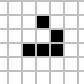
\includegraphics[width=0.15\textwidth]{set2/glider/Game_of_life_animated_glider_wps图片_1.jpg}
          }
          \subfigure{
            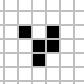
\includegraphics[width=0.15\textwidth]{set2/glider/Game_of_life_animated_glider_wps图片_5.jpg}
          }
          \subfigure{
            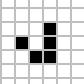
\includegraphics[width=0.15\textwidth]{set2/glider/Game_of_life_animated_glider_wps图片_8.jpg}
          }
          \caption{\textbf{滑翔机(每四步平移一格)}}
        \end{figure}
  \end{itemize}
\end{itemize}

\hypertarget{ux590dux6742ux6a21ux5f0fux7684ux6539ux8fdb}{%
\subsection{复杂模式的改进}\label{ux590dux6742ux6a21ux5f0fux7684ux6539ux8fdb}}

\begin{itemize}
\tightlist
\item
  可以拓展接口,使得参数可以自定义
\item
  可以探索更多的竞争力、独立度、扩散常数、竞争力阈值(用于判断因拥挤而死的阈值)的参数组合,使得游戏更具有可玩性
\item
  可以探索在特定参数下,复杂生命游戏的特殊结构,类似于简单生命游戏中的静物、振荡器、滑翔机等
\end{itemize}

\hypertarget{ux5355ux7247ux673aux7684ux6539ux8fdb}{%
\subsection{单片机的改进}\label{ux5355ux7247ux673aux7684ux6539ux8fdb}}

\begin{itemize}
\tightlist
\item
  可以使用其他功能更为全面的单片机实现生命游戏,以及复杂生命游戏的参数自定义化,例如AVR单片机、PIC单片机、MSP430单片机等等
\end{itemize}

    \hypertarget{ux5c0fux7ec4ux5206ux5de5ux5408ux4f5c}{%
\section{小组分工合作}\label{ux5c0fux7ec4ux5206ux5de5ux5408ux4f5c}}

\begin{table}[h]
    \centering
    \caption{\textbf{小组分工合作\\}}
    \begin{tabularx}{\linewidth}{>{\centering\arraybackslash}m{2cm} >{\centering\arraybackslash}X}
        \hline
        姓名 & 工作 \\
        \hline
        \textbf{王子宸} & 源代码编写与调试,实习报告撰写,海报制作,视频剪辑\\
        
        \textbf{石城玮} & 游戏思路提供与参数设置,源代码调试与游戏测试,视频素材制作\\
        \hline
    \end{tabularx}
\end{table}


\end{document}
